\level{1}{Chuck}
    \level{2}{Specifica dei componenti}
        Nella presente sezione è stata riportata e documentata la progettazione di dettaglio del \insglo{prodotto} \insglo{Chuck}. Si noti che tale progettazione deriva direttamente dalla progettazione architetturale che può essere trovata all'interno del documento \insdoc{Specifica Tecnica v5.00}. I risultati ottenuti sono stati organizzati e presentati secondo la seguente struttura:
        \begin{enumerate}
            \item vengono innanzitutto presentate le varie classi che sono state individuate. Per ognuna di esse si indica il nome, il tipo, l'eventuale astrattezza, la visibilità e il fatto che estenda altre classi oppure no. In aggiunta a ciò, viene presentata una descrizione completa del ruolo e delle responsabilità della classe oltre a una documentazione completa riguardante tutti gli attributi e i metodi presenti all'interno.
            \item in secondo luogo vengono presentati i diagrammi di sequenza, che hanno lo scopo di descrivere scenari (determinate sequenze di azioni in cui tutte le scelte sono già state effettuate). Essi vengono usati per descrivere le relazioni che intercorrono, in termini di messaggi, tra attori, oggetti ed entità del sistema \insglo{Chuck}.
        \end{enumerate}
        Le regole che sono state rispettate, gli strumenti che sono stati usati e le procedure che sono state effettuate possono essere trovate all'interno del documento \insdoc{Norme di Progetto v6.00}.
        \level{3}{Gerarchie presenti in Norris}
            Di seguito vengono elencate tutte le gerarchie presenti in Chuck per fornire in forma visiva tutti i tipi implementati/estesi dalle singole componenti.
            \begin{itemize}
                \item Gerarchie in Model::NorrisChart \\
                    La seguente gerarchia rappresenta tutte le tipologie di chart utilizzate in Chuck.
                    \begin{figure}[H]
                        \centering
                        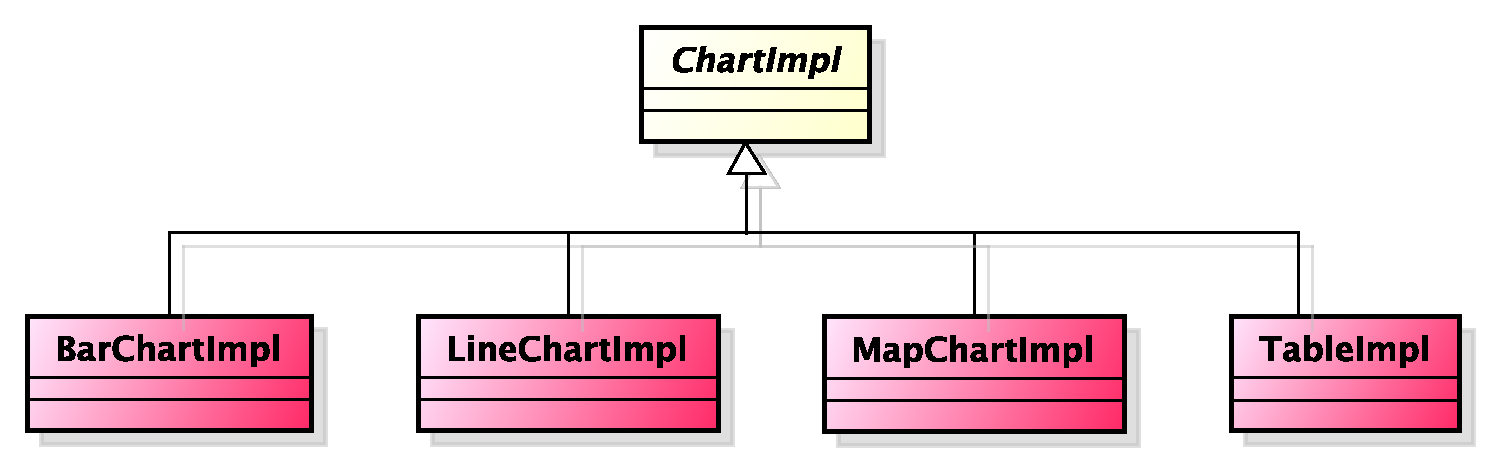
\includegraphics[width=1\textwidth]{DefinizioneDiProdotto/Pics/Gerarchie/ModelChartImpl.pdf}
                        \caption{Diagramma gerarchia ChartImpl in Chuck Model::NorrisChart }
                    \end{figure}
                    La seguente gerarchia rappresenta tutte le tipologie di chart factory che permettono la creazione dei vari chart.
                    \begin{figure}[H]
                        \centering
                        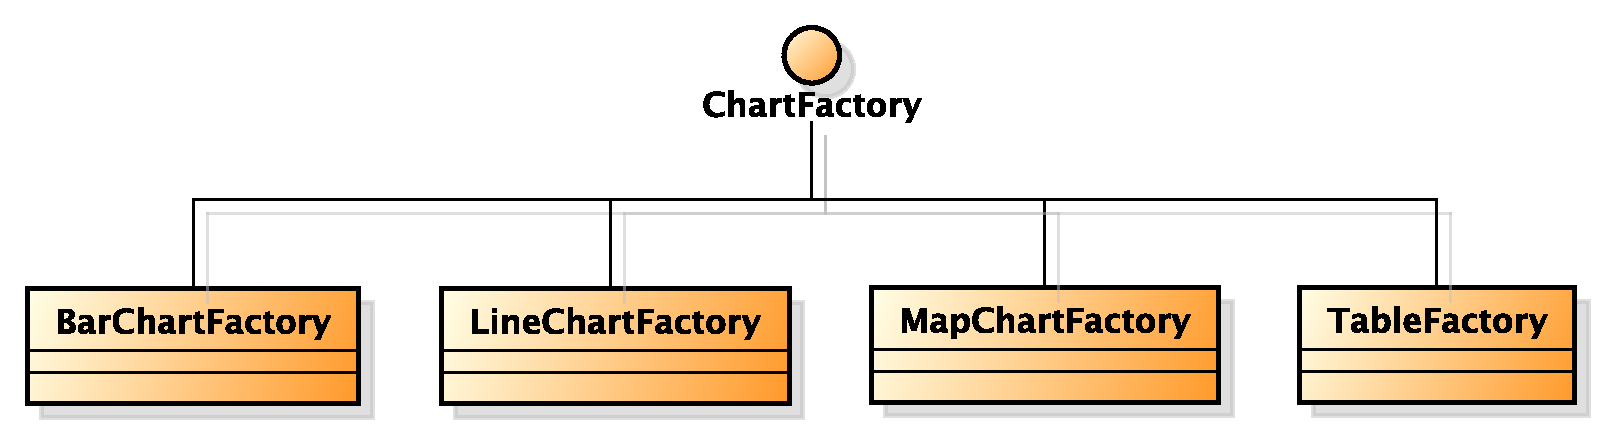
\includegraphics[width=1\textwidth]{DefinizioneDiProdotto/Pics/Gerarchie/ModelFactory.pdf}
                        \caption{Diagramma gerarchia ChartFactory in Chuck Model::NorrisChart}
                    \end{figure}
                    La seguente gerarchia rappresenta tutte le tipologie di updater che possono esser utilizzate per aggiornare un chart.
                    \begin{figure}[H]
                        \centering
                        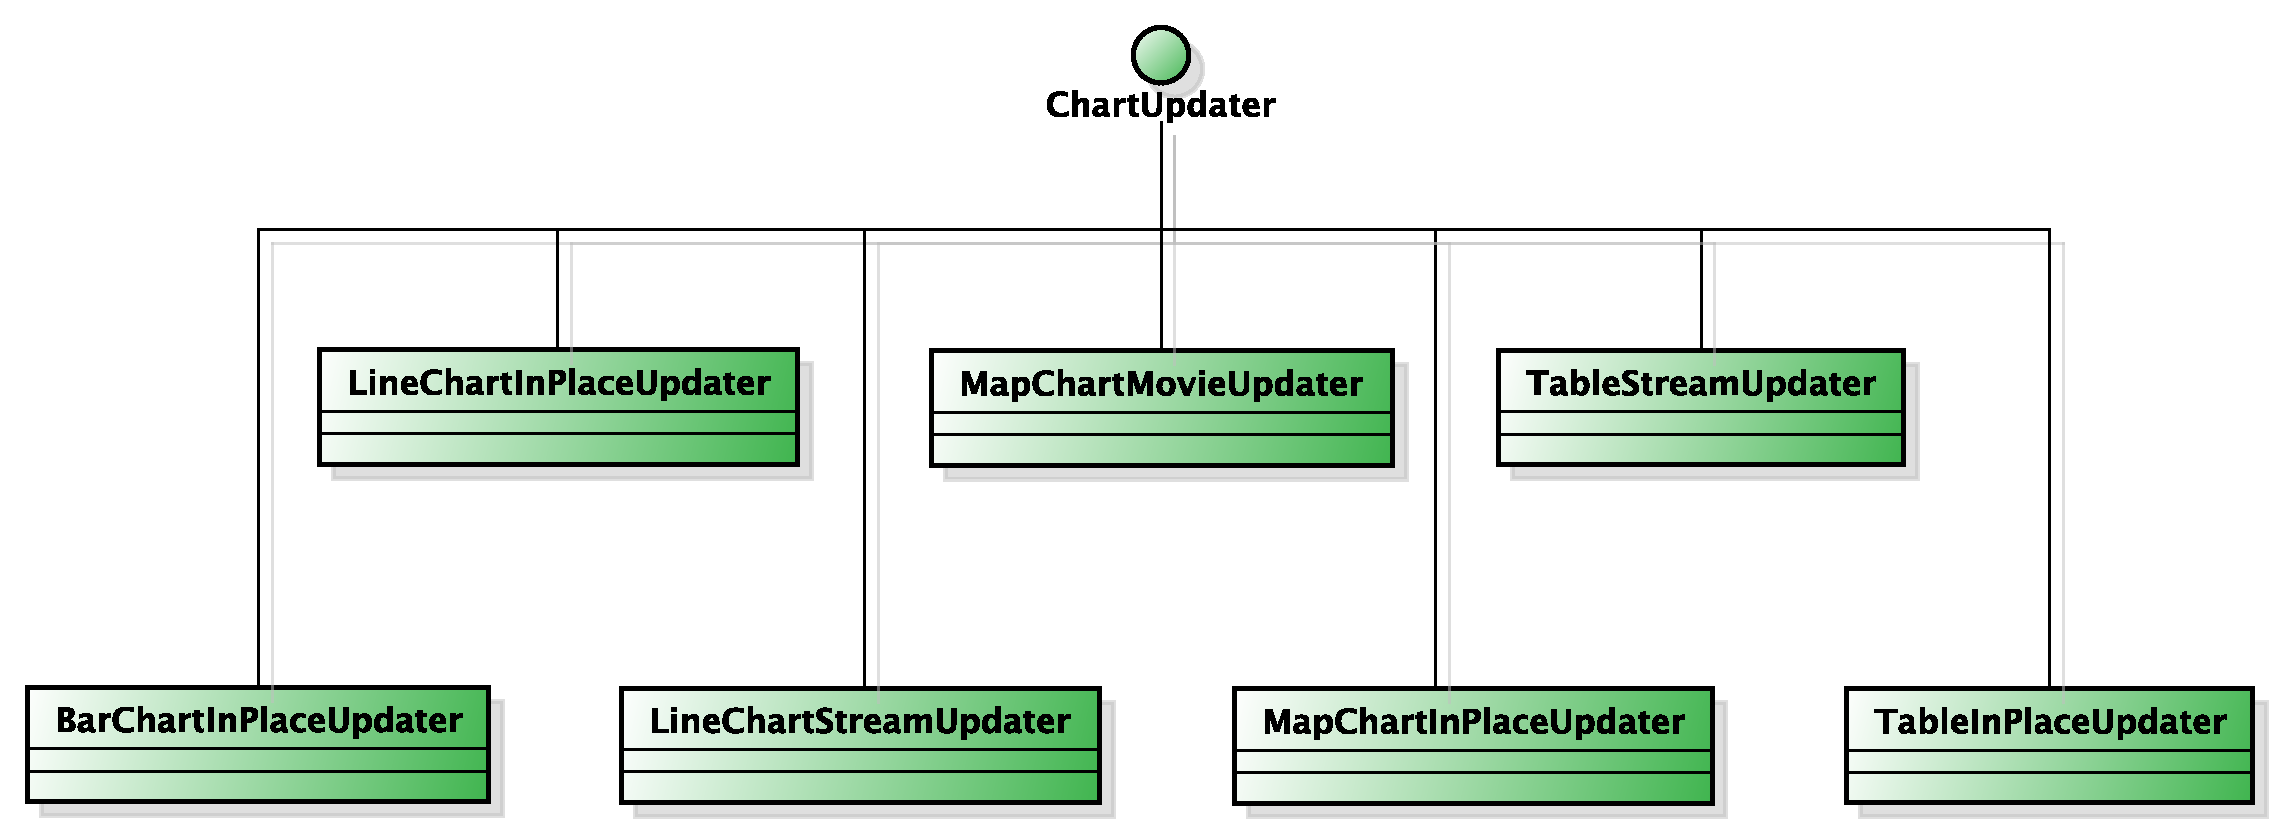
\includegraphics[width=1\textwidth]{DefinizioneDiProdotto/Pics/Gerarchie/ModelUpdater.pdf}
                        \caption{Diagramma gerarchia Updater in Chuck Model::NorrisChart }
                    \end{figure}
                \item Gerarchie in Model::Services \\
                    La seguente gerarchia rappresenta i servizi utilizzati in Chuck.
                    \begin{figure}[H]
                        \centering
                        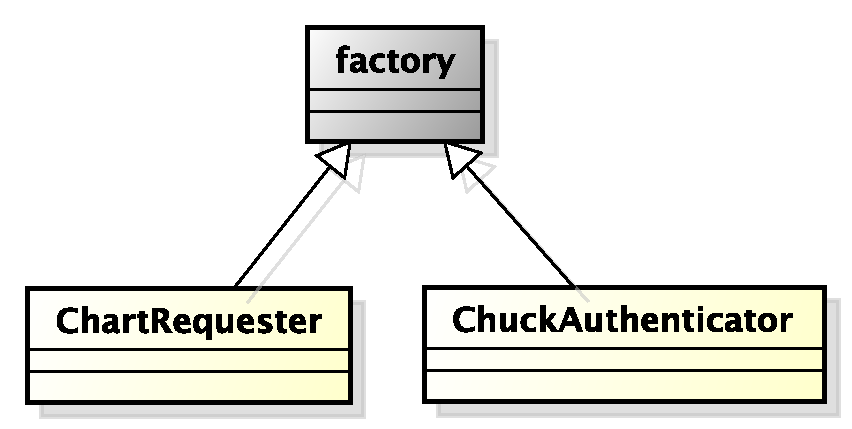
\includegraphics[width=1\textwidth]{DefinizioneDiProdotto/Pics/Gerarchie/ChuckService.pdf}
                        \caption{Diagramma gerarchia dei services in Chuck Model::Services}
                    \end{figure}
                \item Gerarchie in ViewModel \\
                    La seguente gerarchia rappresenta tutte le view-model utilizzate in Chuck.
                    \begin{figure}[H]
                        \centering
                        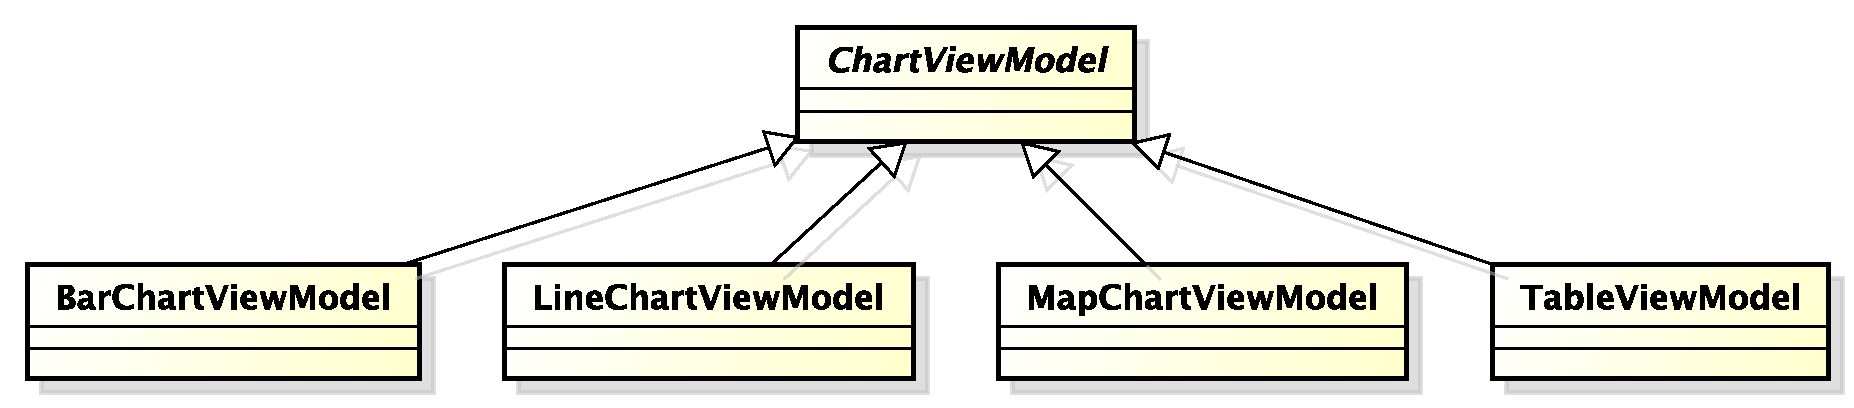
\includegraphics[width=1\textwidth]{DefinizioneDiProdotto/Pics/Gerarchie/ChuckViewModel.pdf}
                        \caption{Diagramma gerarchia dei view-model in Chuck ViewModel}
                    \end{figure}
                \item Gerarchie in Directive \\
                    La seguente gerarchia rappresenta le varie directive utilizzate in Chuck.
                    \begin{figure}[H]
                        \centering
                        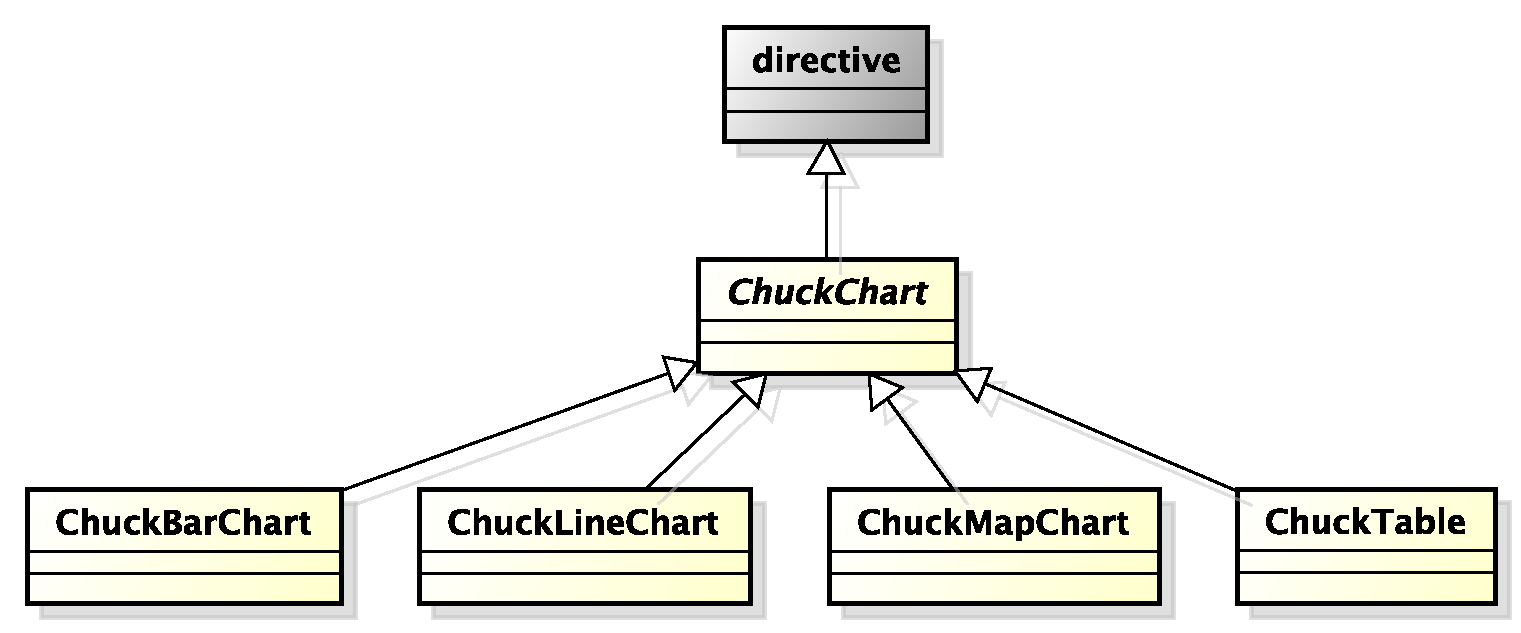
\includegraphics[width=1\textwidth]{DefinizioneDiProdotto/Pics/Gerarchie/ChuckDirective.pdf}
                        \caption{Diagramma gerarchia delle directive in Chuck Directive}
                    \end{figure}
                \item Gerarchie in View \\
                    La seguente gerarchia rappresenta le varie view utilizzate in Chuck.
                    \begin{figure}[H]
                        \centering
                        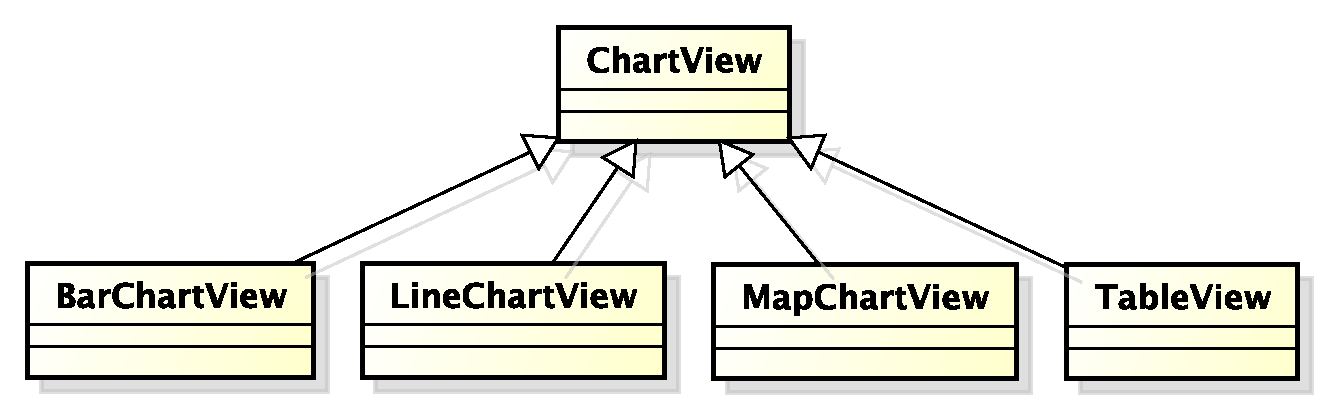
\includegraphics[width=1\textwidth]{DefinizioneDiProdotto/Pics/Gerarchie/ChuckView.pdf}
                        \caption{Diagramma gerarchia delle view in Chuck View}
                    \end{figure}
            \end{itemize}

        \level{3}{Classi}
            In tale sezione sono riportate delle descrizioni dettagliate delle classi individuate all'interno del documento \insdoc{Specifica Tecnica v4.00}. Tali classi sono presentate e organizzate in modo gerarchico, mantenendo una suddivisione per \insglo{package} di appartenenza.
            \level{1}{Chuck}
    \level{2}{Specifica dei componenti}
        Nella presente sezione è stata riportata e documentata la progettazione di dettaglio del \insglo{prodotto} \insglo{Chuck}. Si noti che tale progettazione deriva direttamente dalla progettazione architetturale che può essere trovata all'interno del documento \insdoc{Specifica Tecnica v5.00}. I risultati ottenuti sono stati organizzati e presentati secondo la seguente struttura:
        \begin{enumerate}
            \item vengono innanzitutto presentate le varie classi che sono state individuate. Per ognuna di esse si indica il nome, il tipo, l'eventuale astrattezza, la visibilità e il fatto che estenda altre classi oppure no. In aggiunta a ciò, viene presentata una descrizione completa del ruolo e delle responsabilità della classe oltre a una documentazione completa riguardante tutti gli attributi e i metodi presenti all'interno.
            \item in secondo luogo vengono presentati i diagrammi di sequenza, che hanno lo scopo di descrivere scenari (determinate sequenze di azioni in cui tutte le scelte sono già state effettuate). Essi vengono usati per descrivere le relazioni che intercorrono, in termini di messaggi, tra attori, oggetti ed entità del sistema \insglo{Chuck}.
        \end{enumerate}
        Le regole che sono state rispettate, gli strumenti che sono stati usati e le procedure che sono state effettuate possono essere trovate all'interno del documento \insdoc{Norme di Progetto v6.00}.
        \level{3}{Gerarchie presenti in Chuck}
            Di seguito vengono elencate tutte le gerarchie presenti in \insglo{Chuck} per fornire in forma visiva tutti i tipi implementati/estesi dalle singole componenti.
            \begin{itemize}
                \item Gerarchie in Model::NorrisChart \\
                    La seguente gerarchia rappresenta tutte le tipologie di chart utilizzate in \insglo{Chuck}.
                    \begin{figure}[H]
                        \centering
                        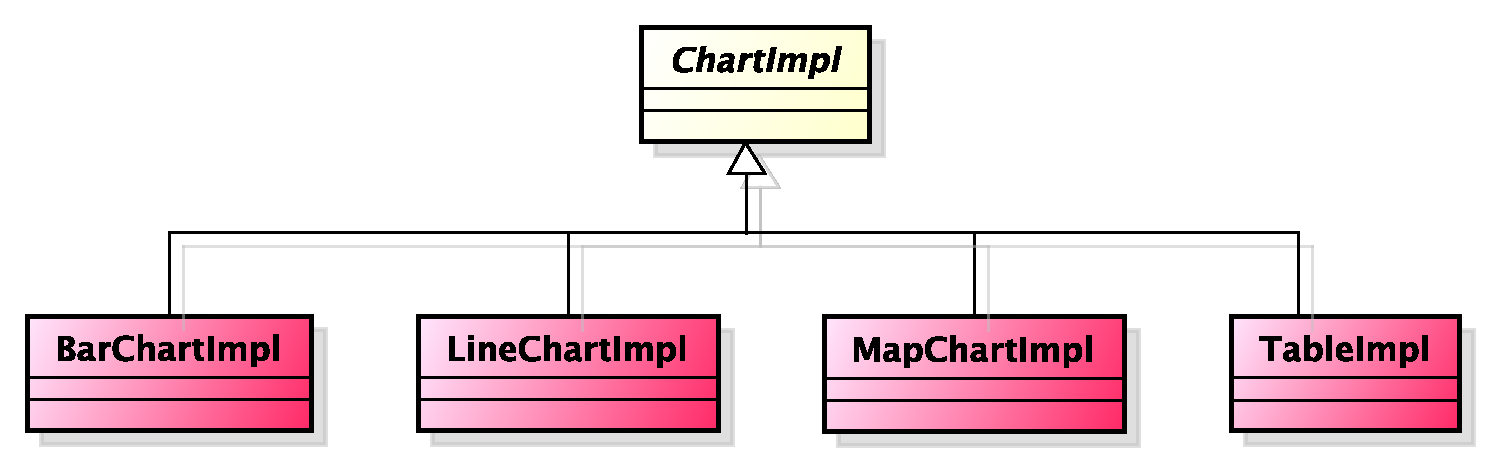
\includegraphics[width=1\textwidth]{DefinizioneDiProdotto/Pics/Gerarchie/ModelChartImpl.pdf}
                        \caption{Diagramma gerarchia ChartImpl in Chuck Model::NorrisChart }
                    \end{figure}
                    La seguente gerarchia rappresenta tutte le tipologie di chart factory che permettono la creazione dei vari chart.
                    \begin{figure}[H]
                        \centering
                        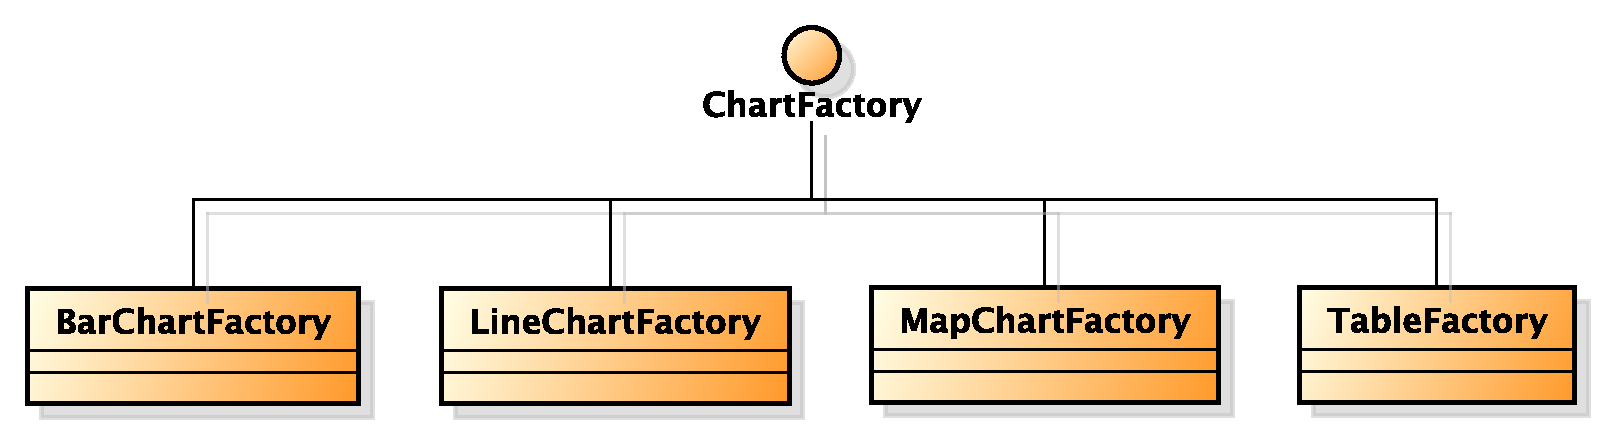
\includegraphics[width=1\textwidth]{DefinizioneDiProdotto/Pics/Gerarchie/ModelFactory.pdf}
                        \caption{Diagramma gerarchia ChartFactory in Chuck Model::NorrisChart}
                    \end{figure}
                    La seguente gerarchia rappresenta tutte le tipologie di updater che possono esser utilizzate per aggiornare un chart.
                    \begin{figure}[H]
                        \centering
                        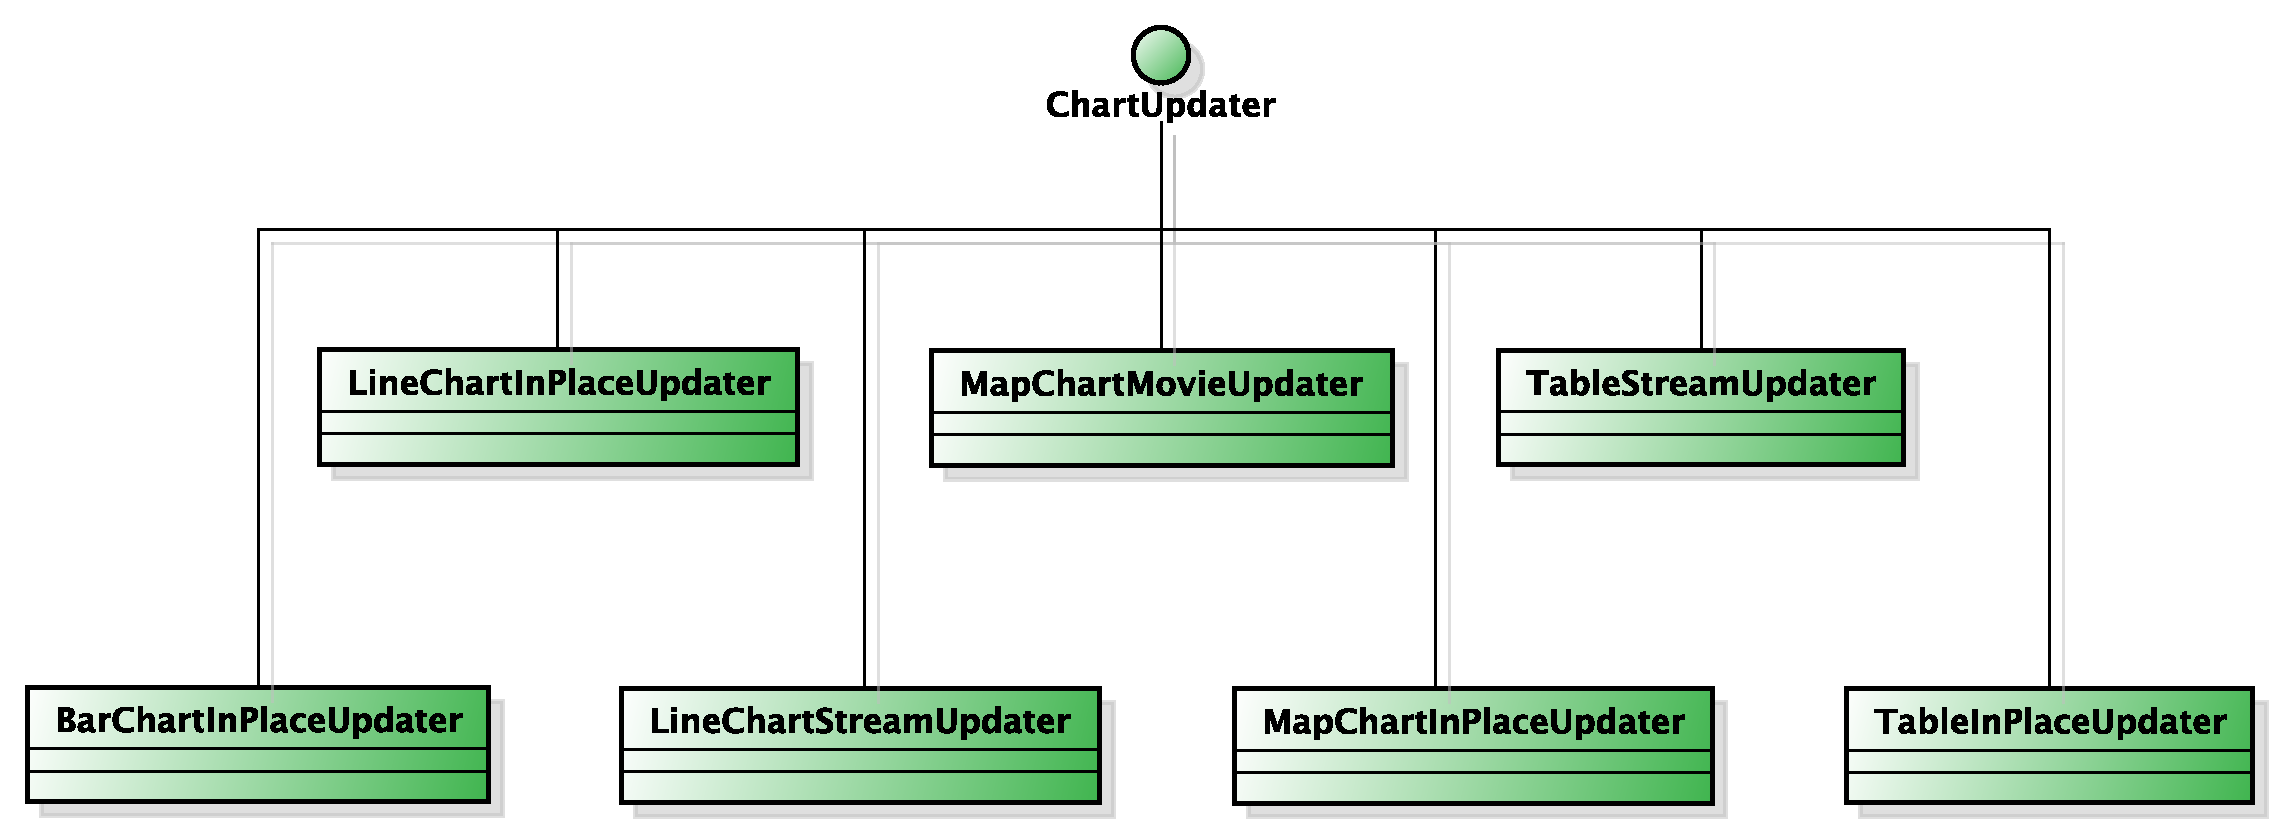
\includegraphics[width=1\textwidth]{DefinizioneDiProdotto/Pics/Gerarchie/ModelUpdater.pdf}
                        \caption{Diagramma gerarchia Updater in Chuck Model::NorrisChart }
                    \end{figure}
                \item Gerarchie in Model::Services \\
                    La seguente gerarchia rappresenta i servizi utilizzati in \insglo{Chuck}.
                    \begin{figure}[H]
                        \centering
                        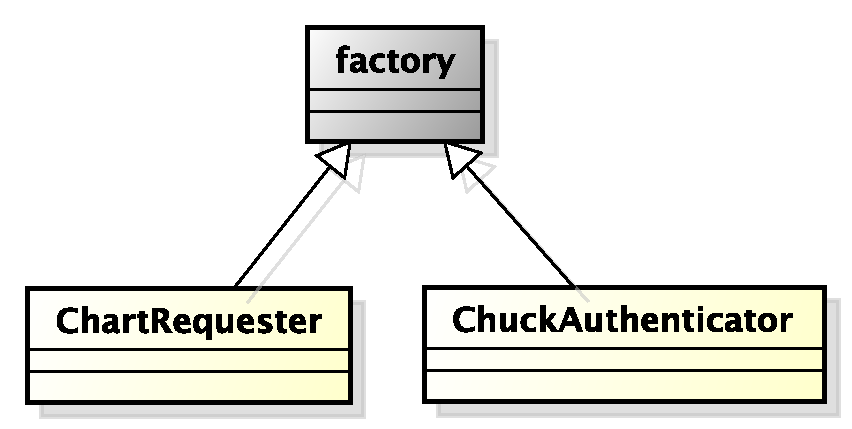
\includegraphics[width=1\textwidth]{DefinizioneDiProdotto/Pics/Gerarchie/ChuckService.pdf}
                        \caption{Diagramma gerarchia dei services in Chuck Model::Services}
                    \end{figure}
                \item Gerarchie in ViewModel \\
                    La seguente gerarchia rappresenta tutte le view-model utilizzate in \insglo{Chuck}.
                    \begin{figure}[H]
                        \centering
                        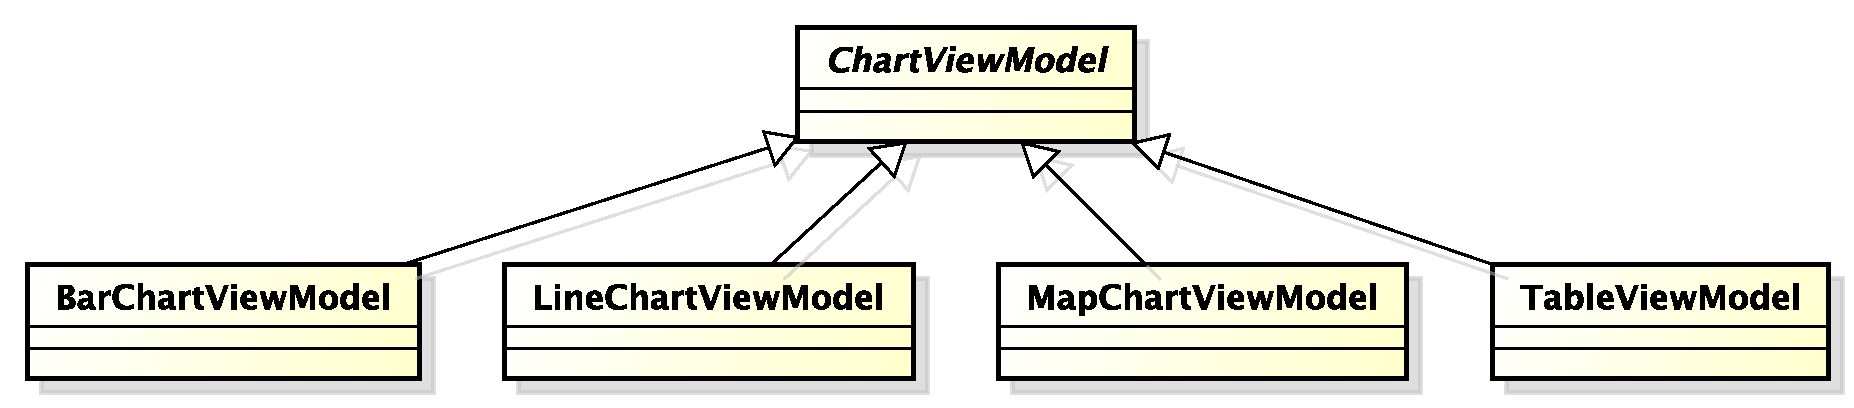
\includegraphics[width=1\textwidth]{DefinizioneDiProdotto/Pics/Gerarchie/ChuckViewModel.pdf}
                        \caption{Diagramma gerarchia dei view-model in Chuck ViewModel}
                    \end{figure}
                \item Gerarchie in Directive \\
                    La seguente gerarchia rappresenta le varie directive utilizzate in \insglo{Chuck}.
                    \begin{figure}[H]
                        \centering
                        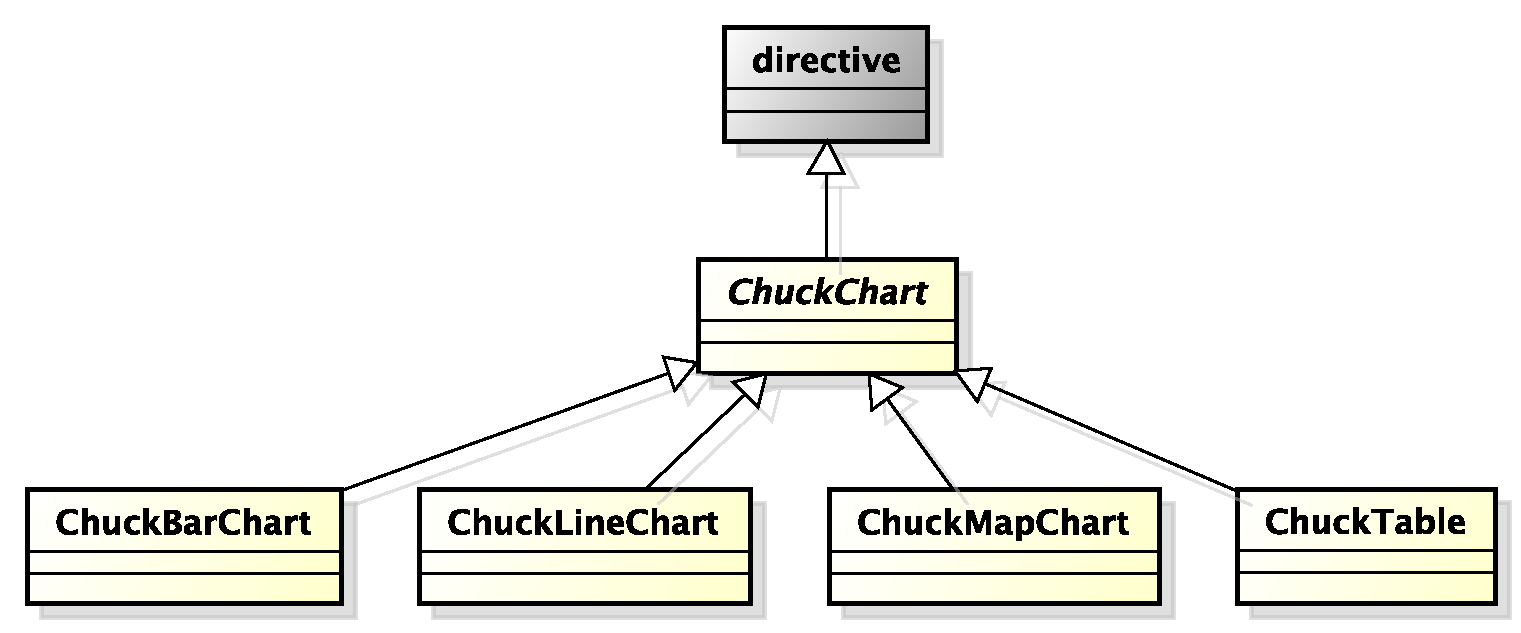
\includegraphics[width=1\textwidth]{DefinizioneDiProdotto/Pics/Gerarchie/ChuckDirective.pdf}
                        \caption{Diagramma gerarchia delle directive in Chuck Directive}
                    \end{figure}
                \item Gerarchie in View \\
                    La seguente gerarchia rappresenta le varie view utilizzate in \insglo{Chuck}.
                    \begin{figure}[H]
                        \centering
                        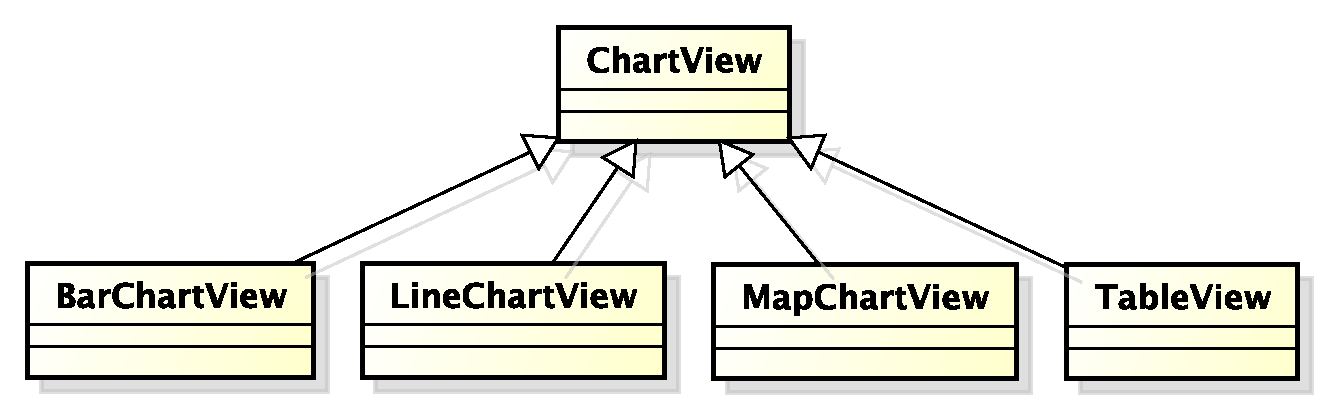
\includegraphics[width=1\textwidth]{DefinizioneDiProdotto/Pics/Gerarchie/ChuckView.pdf}
                        \caption{Diagramma gerarchia delle view in Chuck View}
                    \end{figure}
            \end{itemize}

        \level{3}{Classi}
            In tale sezione sono riportate delle descrizioni dettagliate delle classi individuate all'interno del documento \insdoc{Specifica Tecnica v4.00}. Tali classi sono presentate e organizzate in modo gerarchico, mantenendo una suddivisione per \insglo{package} di appartenenza.
            \level{1}{Chuck}
    \level{2}{Specifica dei componenti}
        Nella presente sezione è stata riportata e documentata la progettazione di dettaglio del \insglo{prodotto} \insglo{Chuck}. Si noti che tale progettazione deriva direttamente dalla progettazione architetturale che può essere trovata all'interno del documento \insdoc{Specifica Tecnica v5.00}. I risultati ottenuti sono stati organizzati e presentati secondo la seguente struttura:
        \begin{enumerate}
            \item vengono innanzitutto presentate le varie classi che sono state individuate. Per ognuna di esse si indica il nome, il tipo, l'eventuale astrattezza, la visibilità e il fatto che estenda altre classi oppure no. In aggiunta a ciò, viene presentata una descrizione completa del ruolo e delle responsabilità della classe oltre a una documentazione completa riguardante tutti gli attributi e i metodi presenti all'interno.
            \item in secondo luogo vengono presentati i diagrammi di sequenza, che hanno lo scopo di descrivere scenari (determinate sequenze di azioni in cui tutte le scelte sono già state effettuate). Essi vengono usati per descrivere le relazioni che intercorrono, in termini di messaggi, tra attori, oggetti ed entità del sistema \insglo{Chuck}.
        \end{enumerate}
        Le regole che sono state rispettate, gli strumenti che sono stati usati e le procedure che sono state effettuate possono essere trovate all'interno del documento \insdoc{Norme di Progetto v6.00}.
        \level{3}{Gerarchie presenti in Chuck}
            Di seguito vengono elencate tutte le gerarchie presenti in \insglo{Chuck} per fornire in forma visiva tutti i tipi implementati/estesi dalle singole componenti.
            \begin{itemize}
                \item Gerarchie in Model::NorrisChart \\
                    La seguente gerarchia rappresenta tutte le tipologie di chart utilizzate in \insglo{Chuck}.
                    \begin{figure}[H]
                        \centering
                        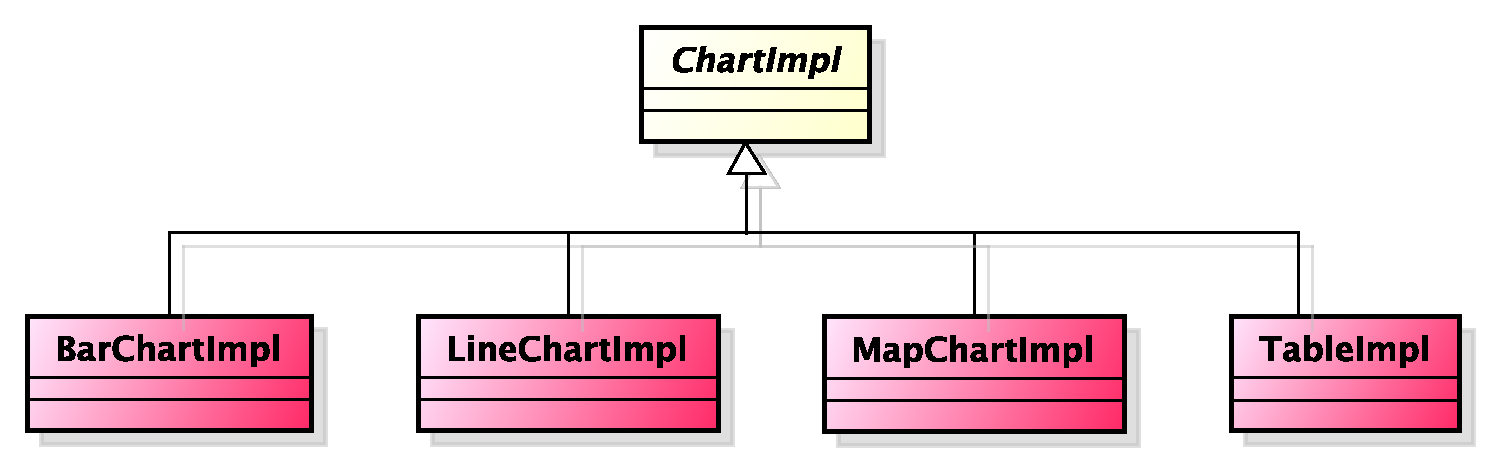
\includegraphics[width=1\textwidth]{DefinizioneDiProdotto/Pics/Gerarchie/ModelChartImpl.pdf}
                        \caption{Diagramma gerarchia ChartImpl in Chuck Model::NorrisChart }
                    \end{figure}
                    La seguente gerarchia rappresenta tutte le tipologie di chart factory che permettono la creazione dei vari chart.
                    \begin{figure}[H]
                        \centering
                        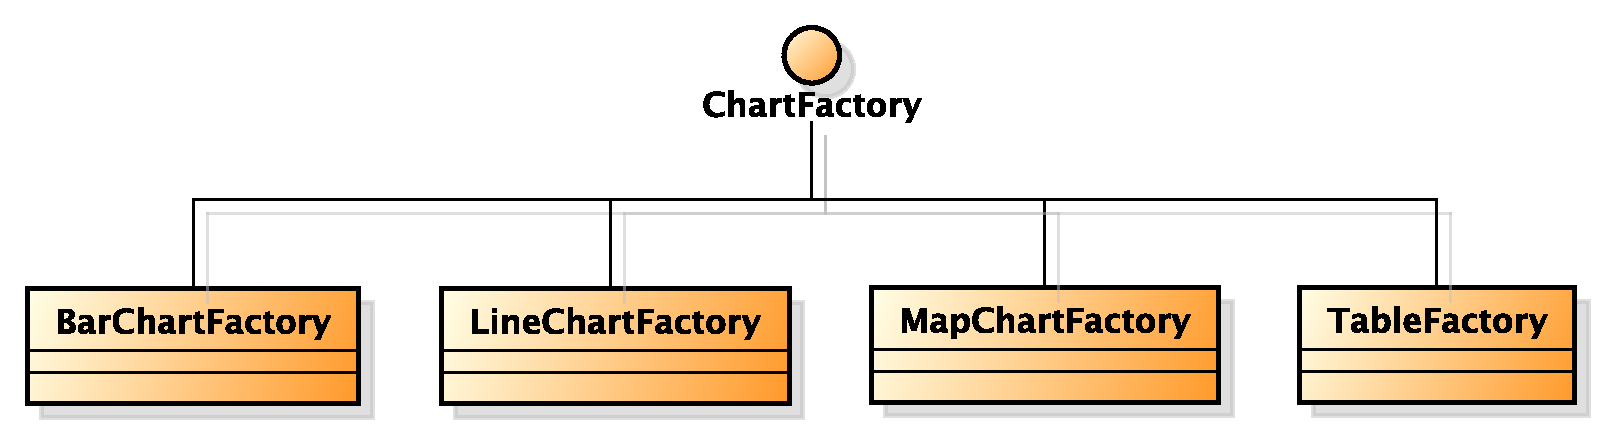
\includegraphics[width=1\textwidth]{DefinizioneDiProdotto/Pics/Gerarchie/ModelFactory.pdf}
                        \caption{Diagramma gerarchia ChartFactory in Chuck Model::NorrisChart}
                    \end{figure}
                    La seguente gerarchia rappresenta tutte le tipologie di updater che possono esser utilizzate per aggiornare un chart.
                    \begin{figure}[H]
                        \centering
                        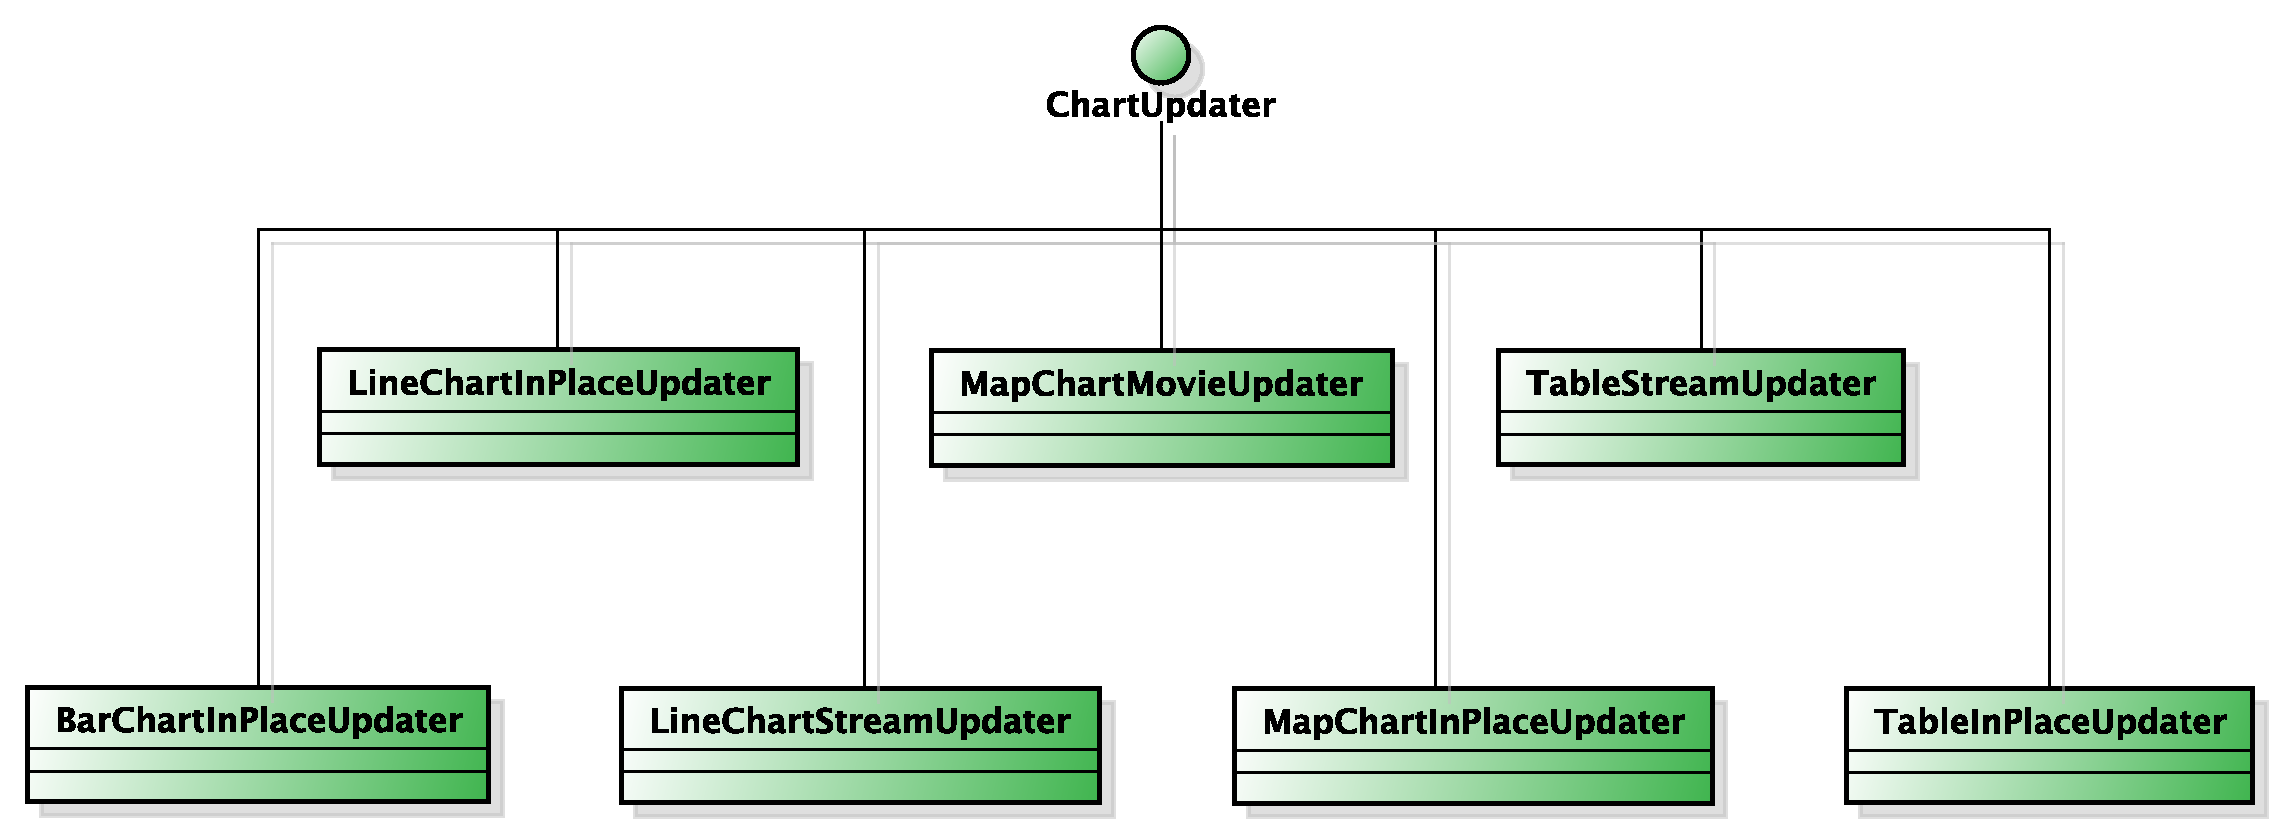
\includegraphics[width=1\textwidth]{DefinizioneDiProdotto/Pics/Gerarchie/ModelUpdater.pdf}
                        \caption{Diagramma gerarchia Updater in Chuck Model::NorrisChart }
                    \end{figure}
                \item Gerarchie in Model::Services \\
                    La seguente gerarchia rappresenta i servizi utilizzati in \insglo{Chuck}.
                    \begin{figure}[H]
                        \centering
                        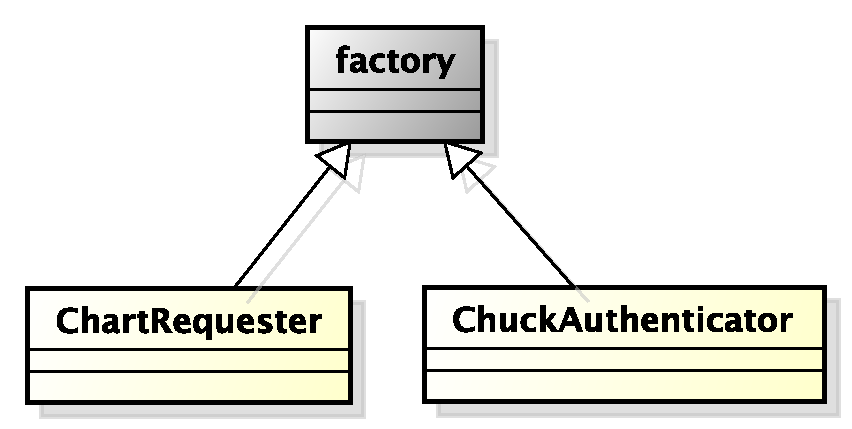
\includegraphics[width=1\textwidth]{DefinizioneDiProdotto/Pics/Gerarchie/ChuckService.pdf}
                        \caption{Diagramma gerarchia dei services in Chuck Model::Services}
                    \end{figure}
                \item Gerarchie in ViewModel \\
                    La seguente gerarchia rappresenta tutte le view-model utilizzate in \insglo{Chuck}.
                    \begin{figure}[H]
                        \centering
                        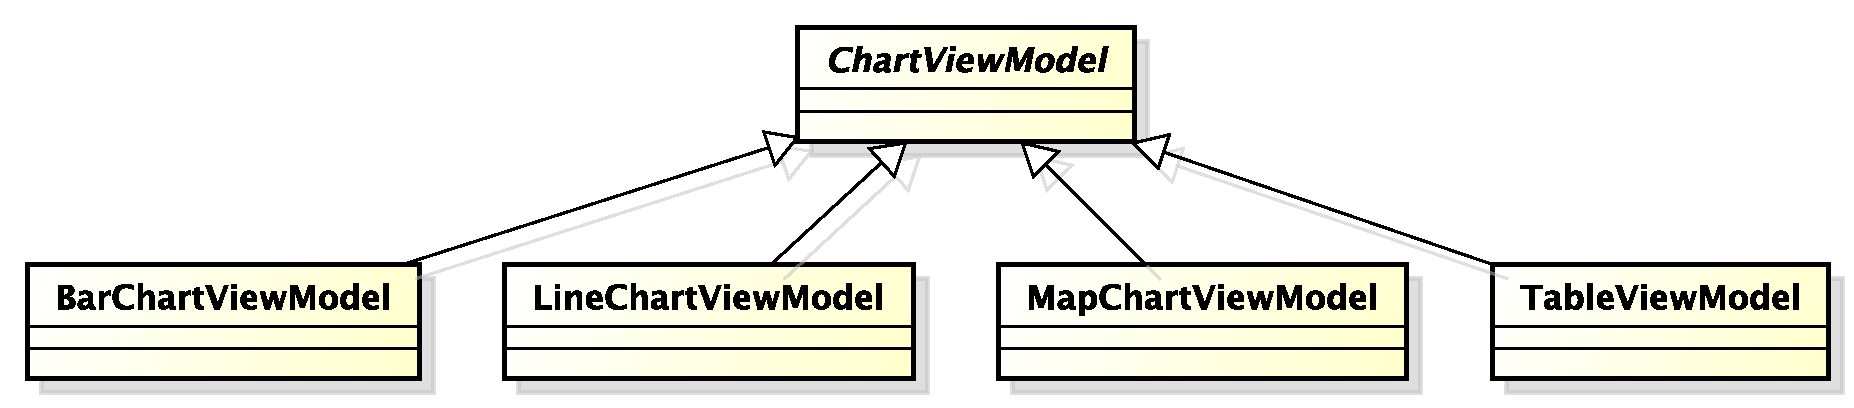
\includegraphics[width=1\textwidth]{DefinizioneDiProdotto/Pics/Gerarchie/ChuckViewModel.pdf}
                        \caption{Diagramma gerarchia dei view-model in Chuck ViewModel}
                    \end{figure}
                \item Gerarchie in Directive \\
                    La seguente gerarchia rappresenta le varie directive utilizzate in \insglo{Chuck}.
                    \begin{figure}[H]
                        \centering
                        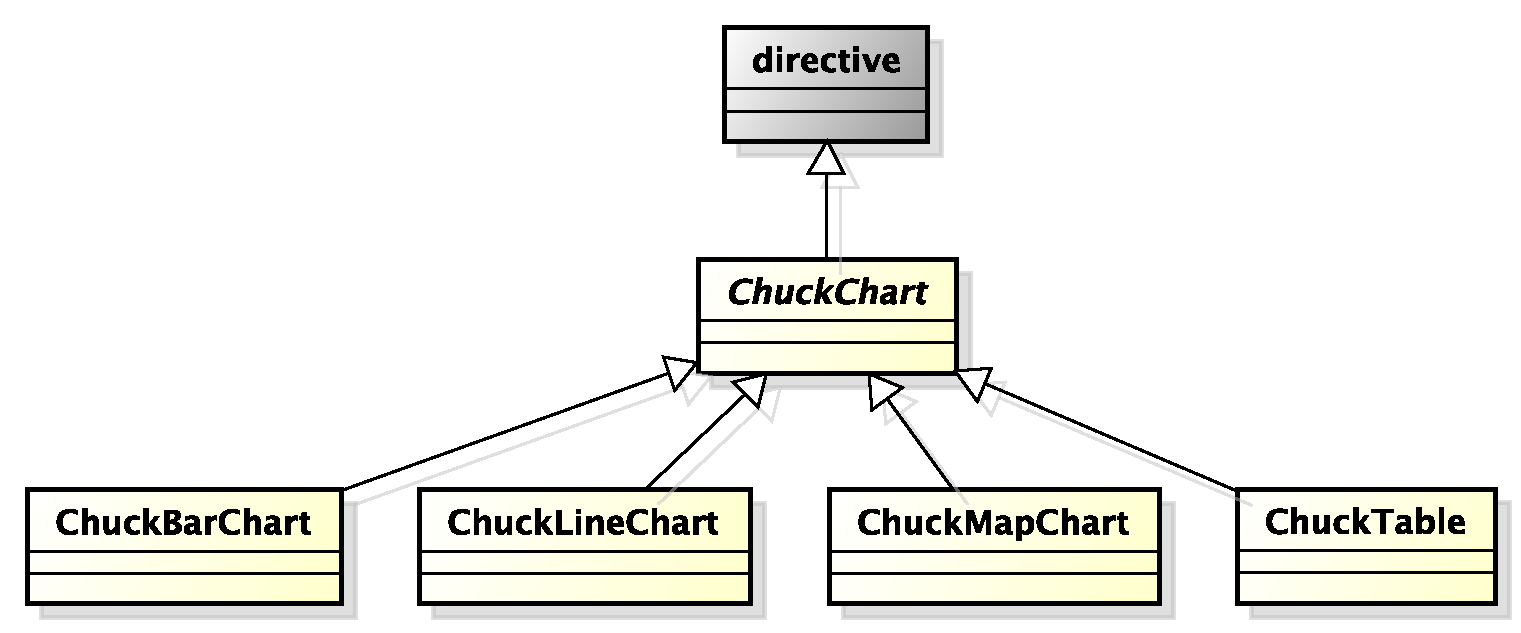
\includegraphics[width=1\textwidth]{DefinizioneDiProdotto/Pics/Gerarchie/ChuckDirective.pdf}
                        \caption{Diagramma gerarchia delle directive in Chuck Directive}
                    \end{figure}
                \item Gerarchie in View \\
                    La seguente gerarchia rappresenta le varie view utilizzate in \insglo{Chuck}.
                    \begin{figure}[H]
                        \centering
                        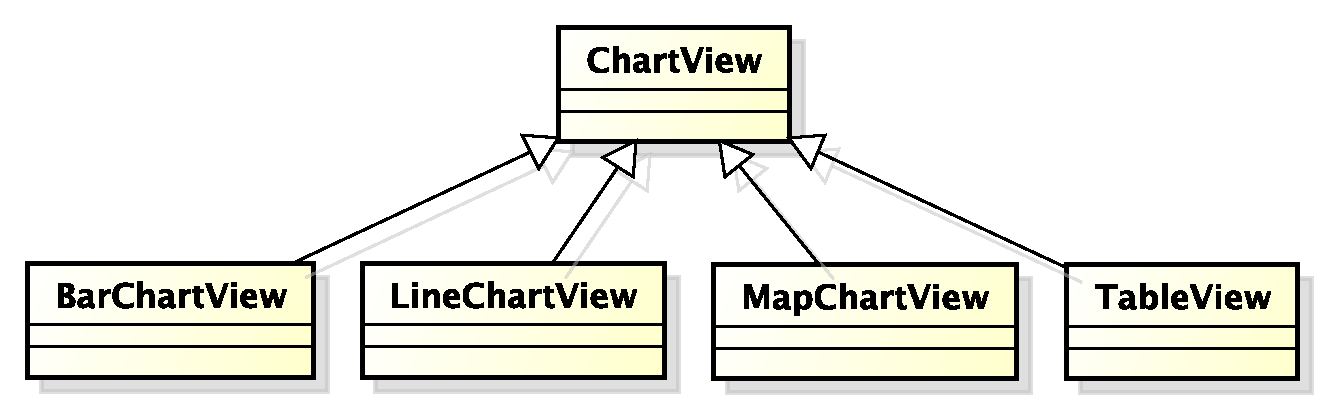
\includegraphics[width=1\textwidth]{DefinizioneDiProdotto/Pics/Gerarchie/ChuckView.pdf}
                        \caption{Diagramma gerarchia delle view in Chuck View}
                    \end{figure}
            \end{itemize}

        \level{3}{Classi}
            In tale sezione sono riportate delle descrizioni dettagliate delle classi individuate all'interno del documento \insdoc{Specifica Tecnica v4.00}. Tali classi sono presentate e organizzate in modo gerarchico, mantenendo una suddivisione per \insglo{package} di appartenenza.
            \level{1}{Chuck}
    \level{2}{Specifica dei componenti}
        Nella presente sezione è stata riportata e documentata la progettazione di dettaglio del \insglo{prodotto} \insglo{Chuck}. Si noti che tale progettazione deriva direttamente dalla progettazione architetturale che può essere trovata all'interno del documento \insdoc{Specifica Tecnica v5.00}. I risultati ottenuti sono stati organizzati e presentati secondo la seguente struttura:
        \begin{enumerate}
            \item vengono innanzitutto presentate le varie classi che sono state individuate. Per ognuna di esse si indica il nome, il tipo, l'eventuale astrattezza, la visibilità e il fatto che estenda altre classi oppure no. In aggiunta a ciò, viene presentata una descrizione completa del ruolo e delle responsabilità della classe oltre a una documentazione completa riguardante tutti gli attributi e i metodi presenti all'interno.
            \item in secondo luogo vengono presentati i diagrammi di sequenza, che hanno lo scopo di descrivere scenari (determinate sequenze di azioni in cui tutte le scelte sono già state effettuate). Essi vengono usati per descrivere le relazioni che intercorrono, in termini di messaggi, tra attori, oggetti ed entità del sistema \insglo{Chuck}.
        \end{enumerate}
        Le regole che sono state rispettate, gli strumenti che sono stati usati e le procedure che sono state effettuate possono essere trovate all'interno del documento \insdoc{Norme di Progetto v6.00}.
        \level{3}{Gerarchie presenti in Chuck}
            Di seguito vengono elencate tutte le gerarchie presenti in \insglo{Chuck} per fornire in forma visiva tutti i tipi implementati/estesi dalle singole componenti.
            \begin{itemize}
                \item Gerarchie in Model::NorrisChart \\
                    La seguente gerarchia rappresenta tutte le tipologie di chart utilizzate in \insglo{Chuck}.
                    \begin{figure}[H]
                        \centering
                        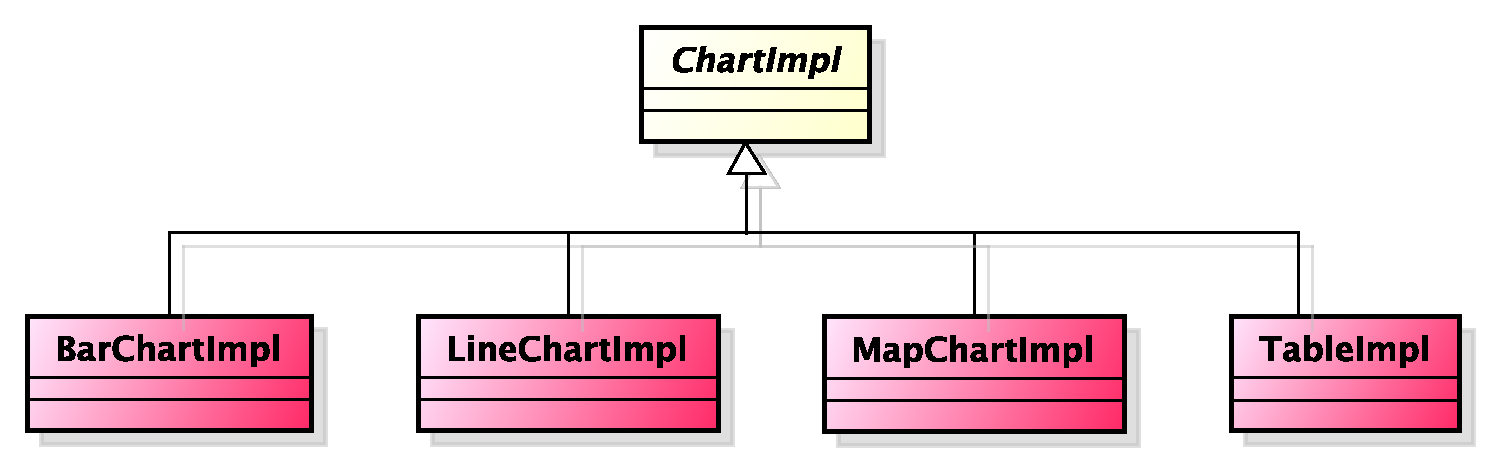
\includegraphics[width=1\textwidth]{DefinizioneDiProdotto/Pics/Gerarchie/ModelChartImpl.pdf}
                        \caption{Diagramma gerarchia ChartImpl in Chuck Model::NorrisChart }
                    \end{figure}
                    La seguente gerarchia rappresenta tutte le tipologie di chart factory che permettono la creazione dei vari chart.
                    \begin{figure}[H]
                        \centering
                        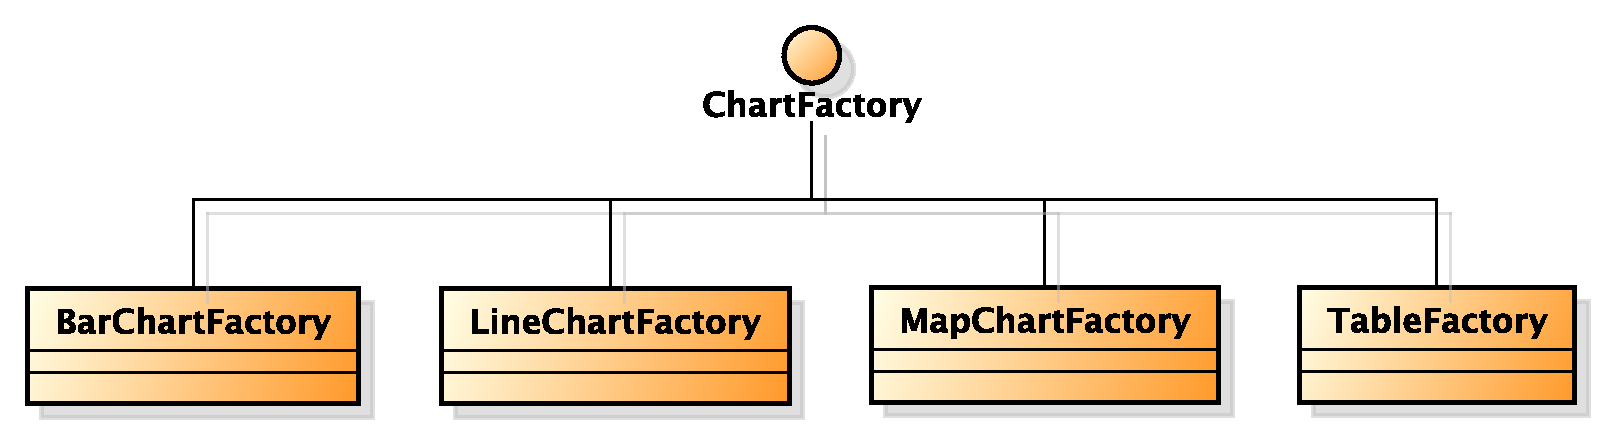
\includegraphics[width=1\textwidth]{DefinizioneDiProdotto/Pics/Gerarchie/ModelFactory.pdf}
                        \caption{Diagramma gerarchia ChartFactory in Chuck Model::NorrisChart}
                    \end{figure}
                    La seguente gerarchia rappresenta tutte le tipologie di updater che possono esser utilizzate per aggiornare un chart.
                    \begin{figure}[H]
                        \centering
                        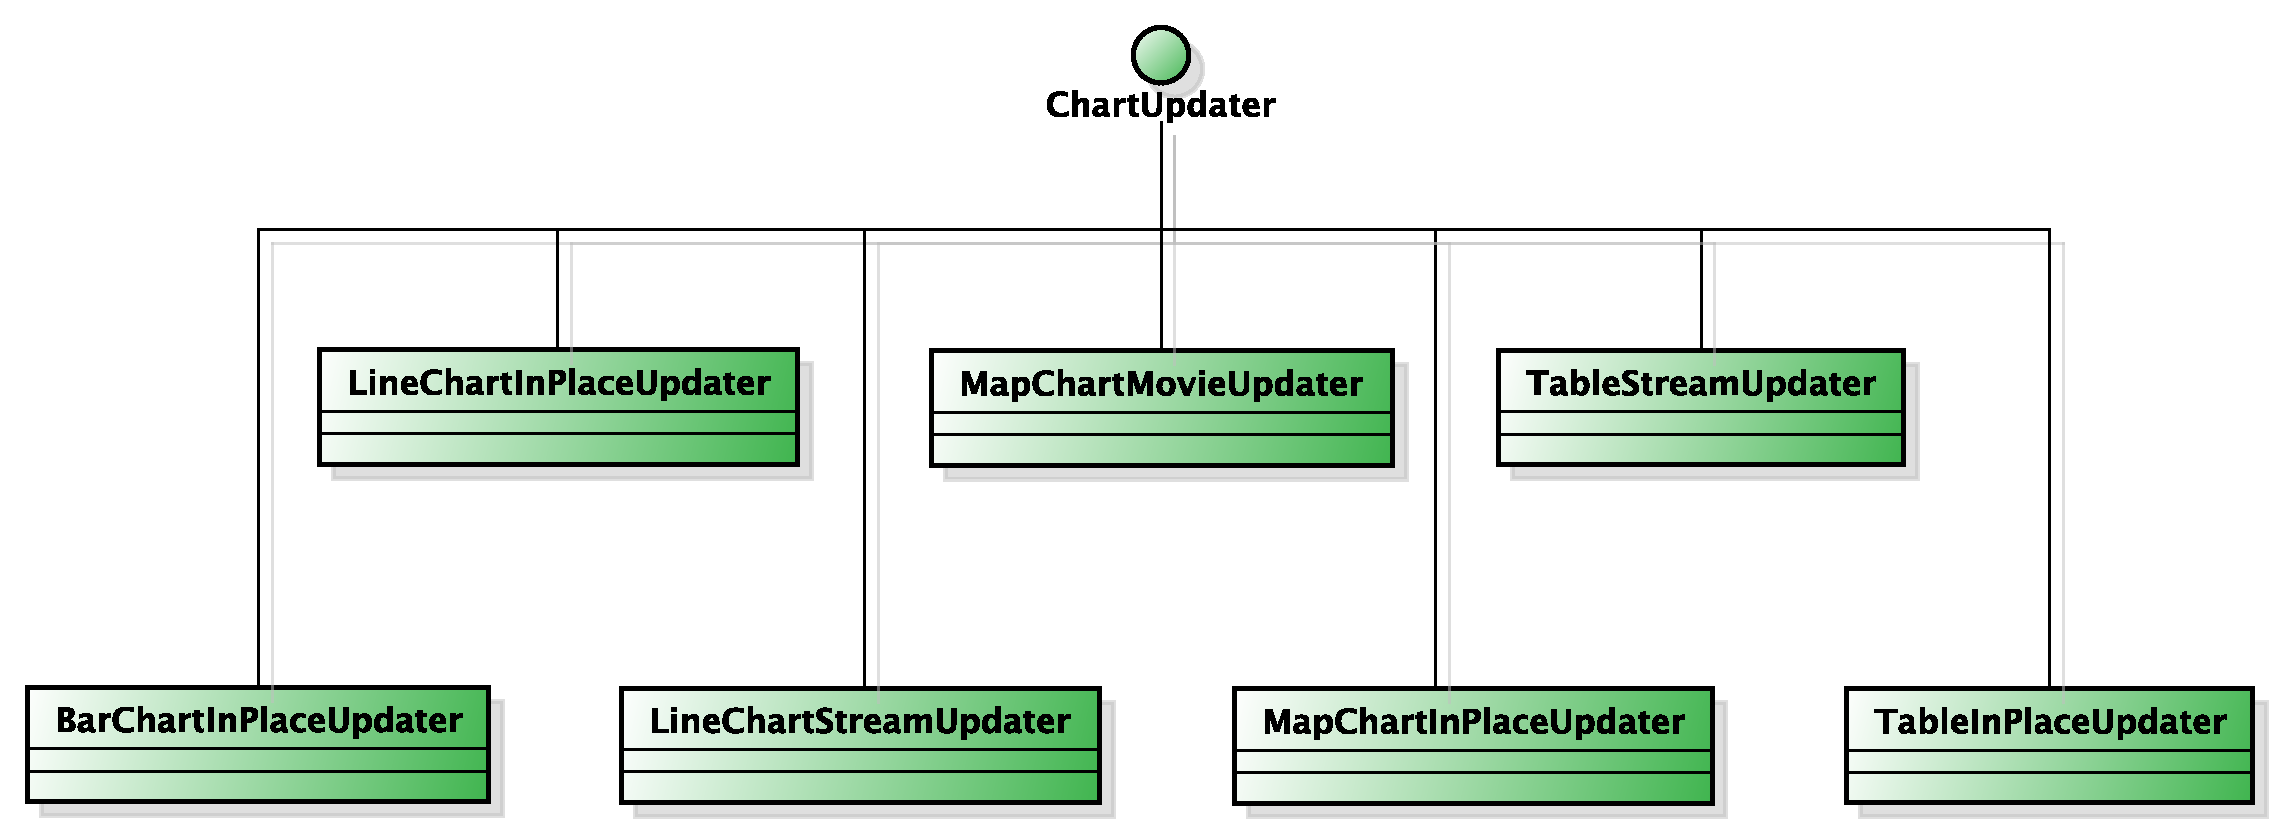
\includegraphics[width=1\textwidth]{DefinizioneDiProdotto/Pics/Gerarchie/ModelUpdater.pdf}
                        \caption{Diagramma gerarchia Updater in Chuck Model::NorrisChart }
                    \end{figure}
                \item Gerarchie in Model::Services \\
                    La seguente gerarchia rappresenta i servizi utilizzati in \insglo{Chuck}.
                    \begin{figure}[H]
                        \centering
                        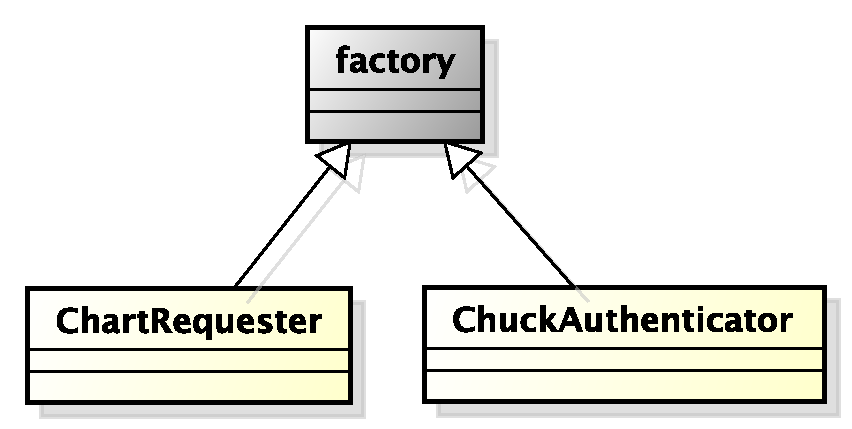
\includegraphics[width=1\textwidth]{DefinizioneDiProdotto/Pics/Gerarchie/ChuckService.pdf}
                        \caption{Diagramma gerarchia dei services in Chuck Model::Services}
                    \end{figure}
                \item Gerarchie in ViewModel \\
                    La seguente gerarchia rappresenta tutte le view-model utilizzate in \insglo{Chuck}.
                    \begin{figure}[H]
                        \centering
                        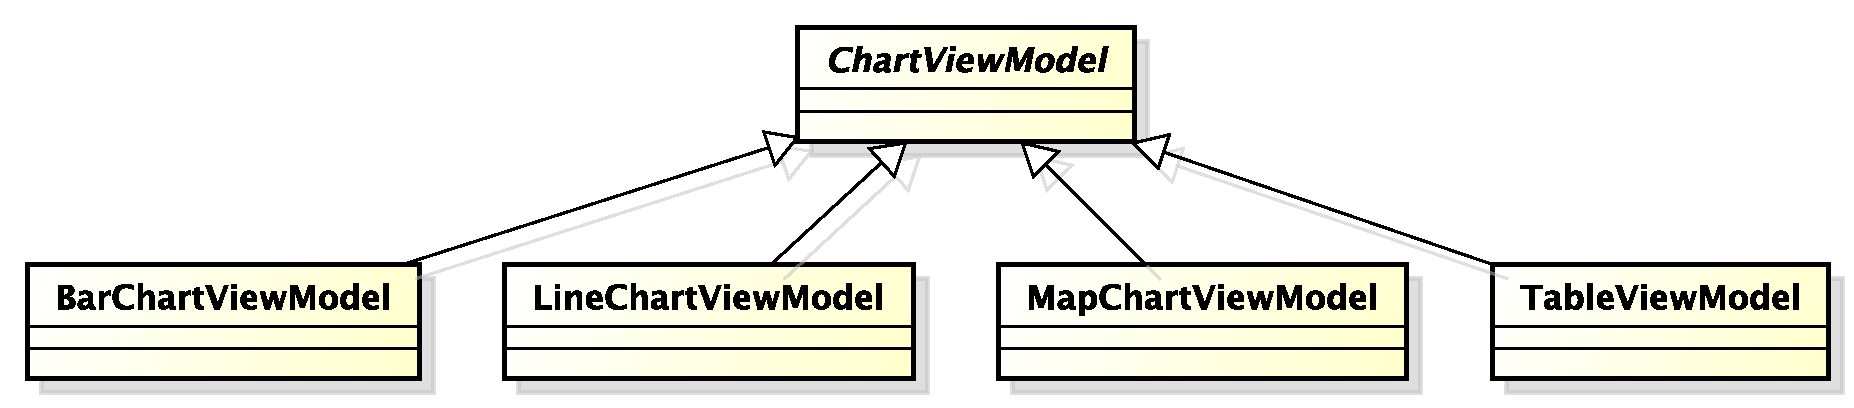
\includegraphics[width=1\textwidth]{DefinizioneDiProdotto/Pics/Gerarchie/ChuckViewModel.pdf}
                        \caption{Diagramma gerarchia dei view-model in Chuck ViewModel}
                    \end{figure}
                \item Gerarchie in Directive \\
                    La seguente gerarchia rappresenta le varie directive utilizzate in \insglo{Chuck}.
                    \begin{figure}[H]
                        \centering
                        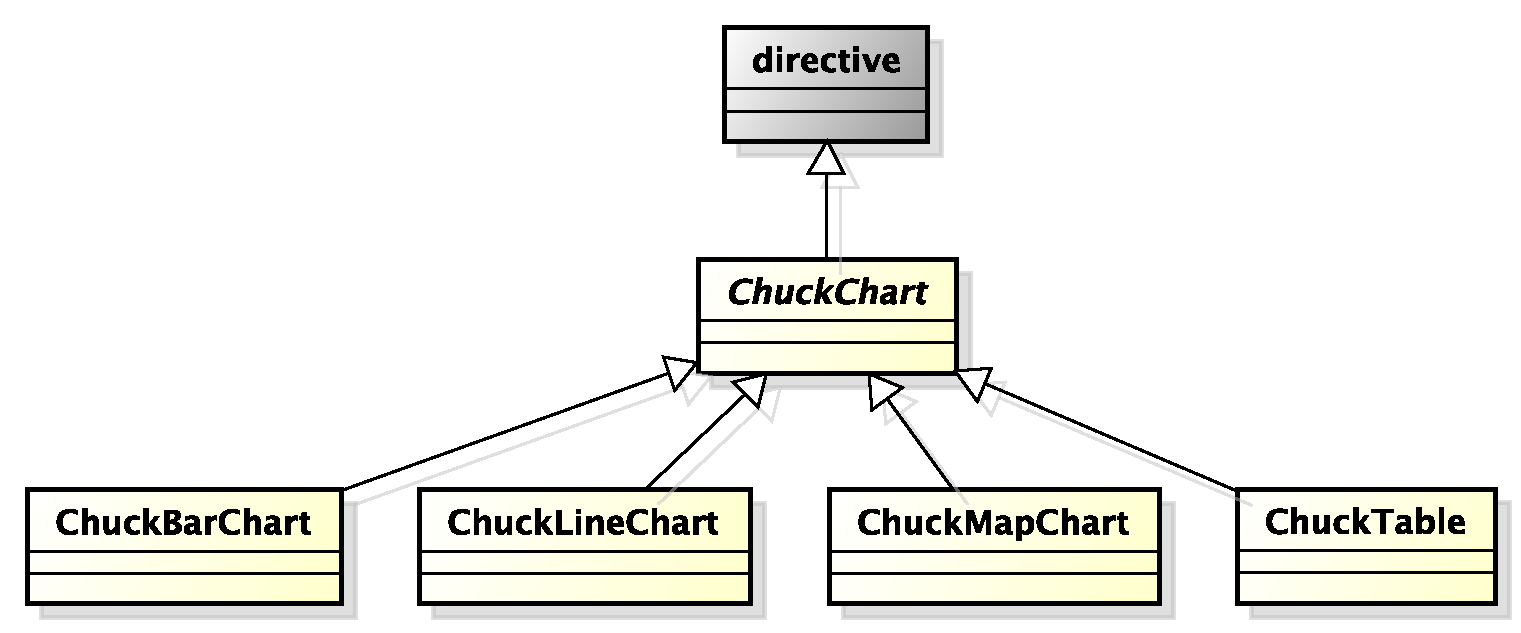
\includegraphics[width=1\textwidth]{DefinizioneDiProdotto/Pics/Gerarchie/ChuckDirective.pdf}
                        \caption{Diagramma gerarchia delle directive in Chuck Directive}
                    \end{figure}
                \item Gerarchie in View \\
                    La seguente gerarchia rappresenta le varie view utilizzate in \insglo{Chuck}.
                    \begin{figure}[H]
                        \centering
                        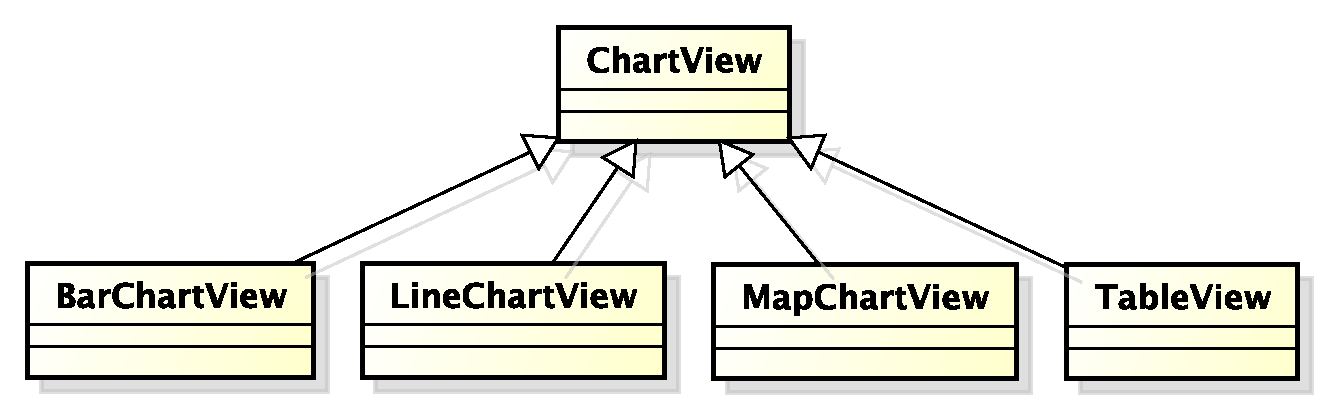
\includegraphics[width=1\textwidth]{DefinizioneDiProdotto/Pics/Gerarchie/ChuckView.pdf}
                        \caption{Diagramma gerarchia delle view in Chuck View}
                    \end{figure}
            \end{itemize}

        \level{3}{Classi}
            In tale sezione sono riportate delle descrizioni dettagliate delle classi individuate all'interno del documento \insdoc{Specifica Tecnica v4.00}. Tali classi sono presentate e organizzate in modo gerarchico, mantenendo una suddivisione per \insglo{package} di appartenenza.
            \input{Classi/Chuck.tex}

    \level{2}{Diagrammi di sequenza}
        In tale sezione vengono presentati i diagrammi di sequenza, che hanno lo scopo di descrivere scenari (determinate sequenze di azioni in cui tutte le scelte sono già state effettuate). Essi vengono usati per descrivere le relazioni che intercorrono, in termini di messaggi, tra attori, oggetti ed entità del sistema \insglo{Chuck}.
        \level{3}{Creazione di un chart}
             Tale diagramma riporta e descrive come viene creato un chart e collegato a quello presente all'interno di una certa istanza di \insglo{Norris}.
            \begin{figure}[H]
                \centering
                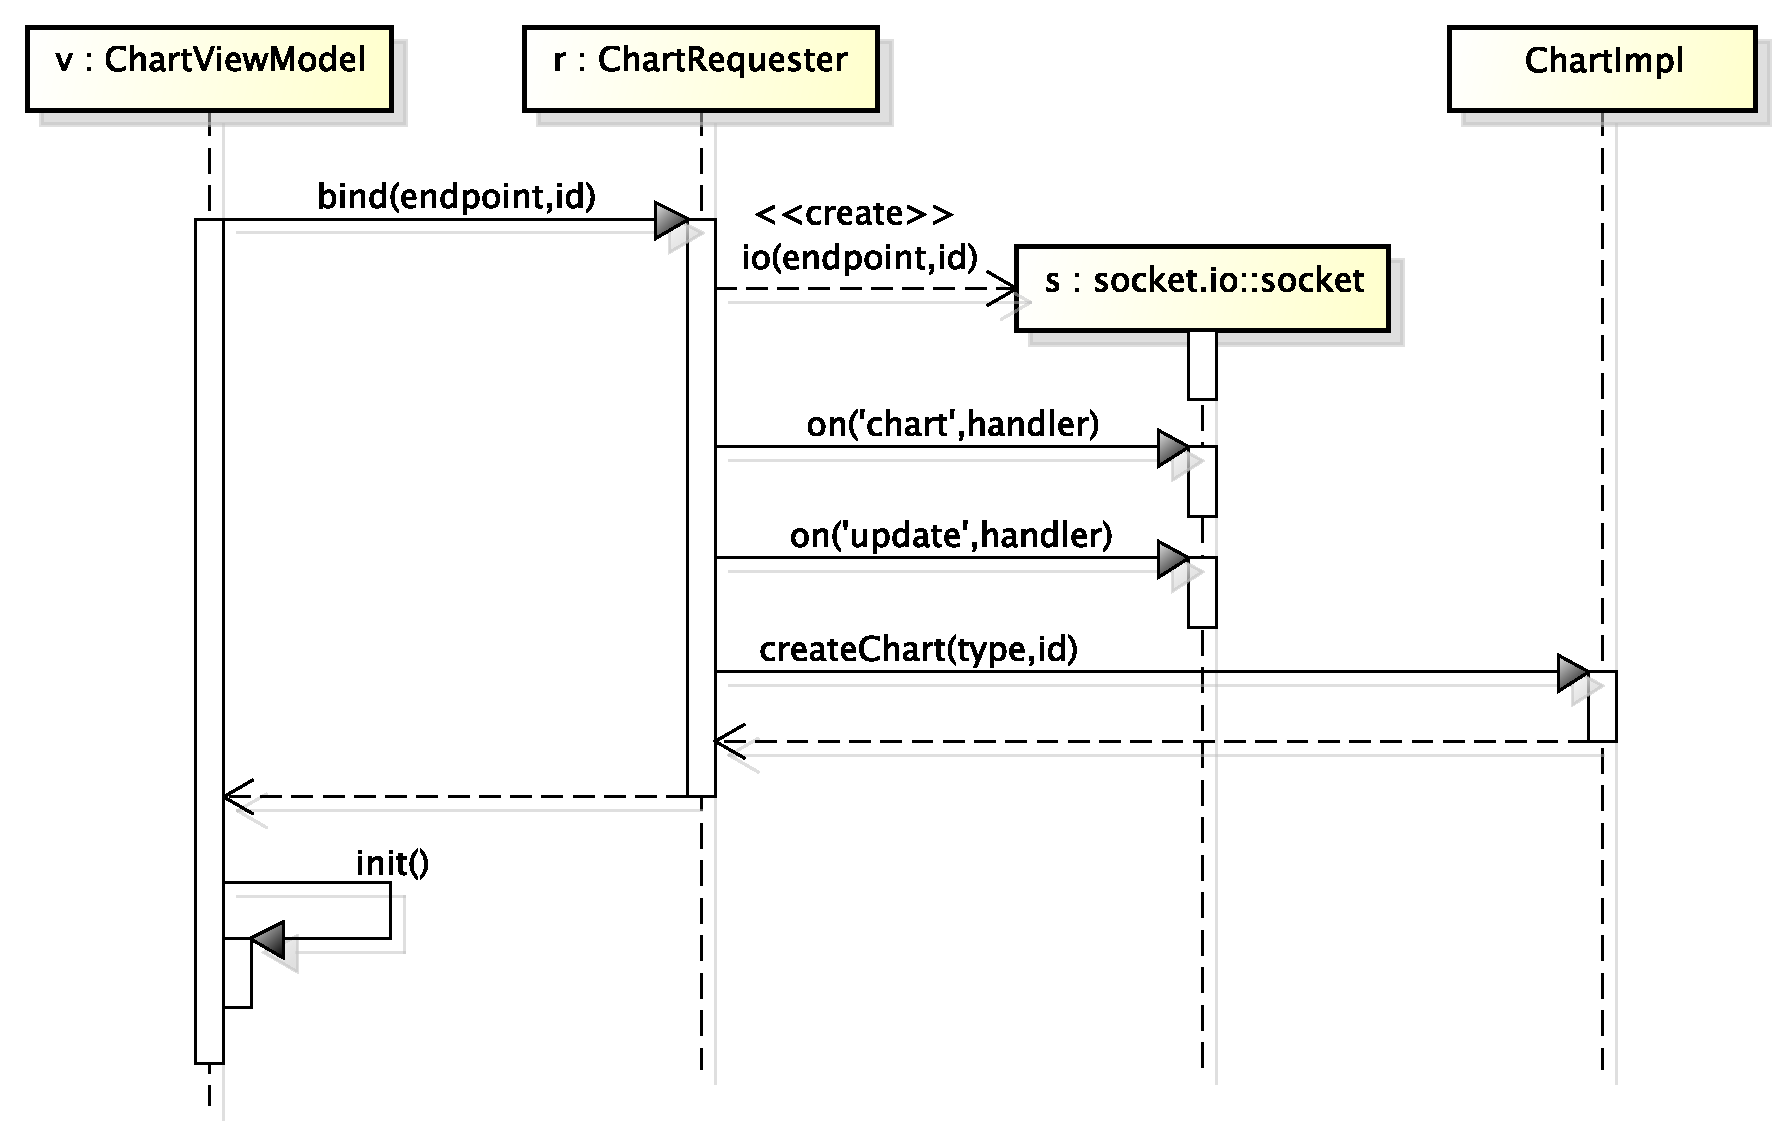
\includegraphics[scale=0.3]{DefinizioneDiProdotto/Pics/ChuckInserimentoChart}
                \caption{Diagramma di sequenza - Chuck, creazione chart}
            \end{figure}
            \begin{enumerate}
                \item ChartViewModel richiede l'ottenimento di un chart specifico presente in una istanza di \insglo{Norris} a ChartRequester;
                \item questo apre il canale socket ed imposta delle \insglo{callback} per gli eventi chart e update;
                \item ricevuto il grafico crea il modello dei dati;
                \item infine ChartViewModel esegue il metodo init che permette di inizializzare la view e visualizzare il Chart secondo i dati memorizzati.
            \end{enumerate}

        \level{3}{Aggiornamento di un chart}
            Tale diagramma descrive come viene aggiornato un chart nel momento in cui arrivano nuovi dati dall'istanza di \insglo{Norris} alla quale il grafico appartiene.
            \begin{figure}[H]
                \centering
                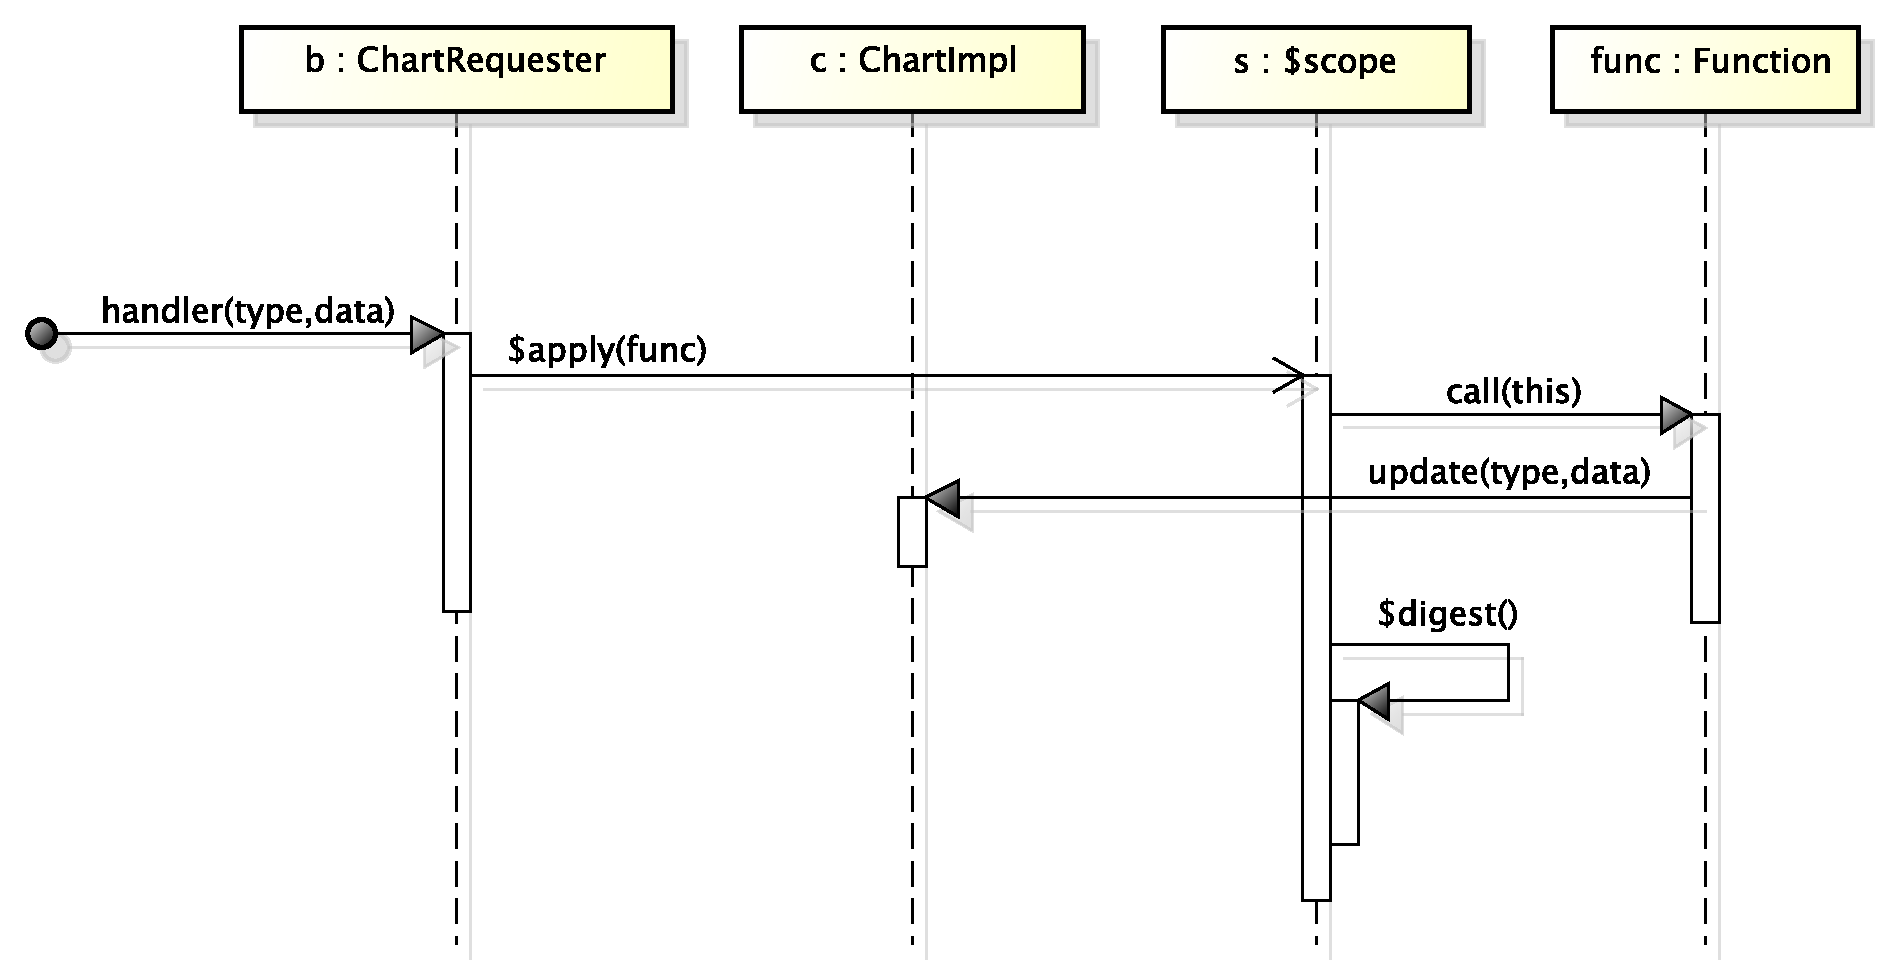
\includegraphics[scale=0.3]{DefinizioneDiProdotto/Pics/ChuckAggiornamentoChart}
                \caption{Diagramma di sequenza - Chuck, aggiornamento chart}
            \end{figure}
            \begin{enumerate}
                \item il messaggio iniziale rappresenta la notifica inviata da ChartRequester da parte di \insglo{Norris} attraverso il canale socket per avvertirlo dell'avvenuto aggiornamento;
                \item ChartRequester aggiorna il modello dei dati;
                \item avverte infine il ChartViewModel di un'avvenuta modifica nel modello richiedendo dunque la renderizzazione dei nuovi dati.
                \item
                \item
                \item
            \end{enumerate}


    \level{2}{Diagrammi di sequenza}
        In tale sezione vengono presentati i diagrammi di sequenza, che hanno lo scopo di descrivere scenari (determinate sequenze di azioni in cui tutte le scelte sono già state effettuate). Essi vengono usati per descrivere le relazioni che intercorrono, in termini di messaggi, tra attori, oggetti ed entità del sistema \insglo{Chuck}.
        \level{3}{Creazione di un chart}
             Tale diagramma riporta e descrive come viene creato un chart e collegato a quello presente all'interno di una certa istanza di \insglo{Norris}.
            \begin{figure}[H]
                \centering
                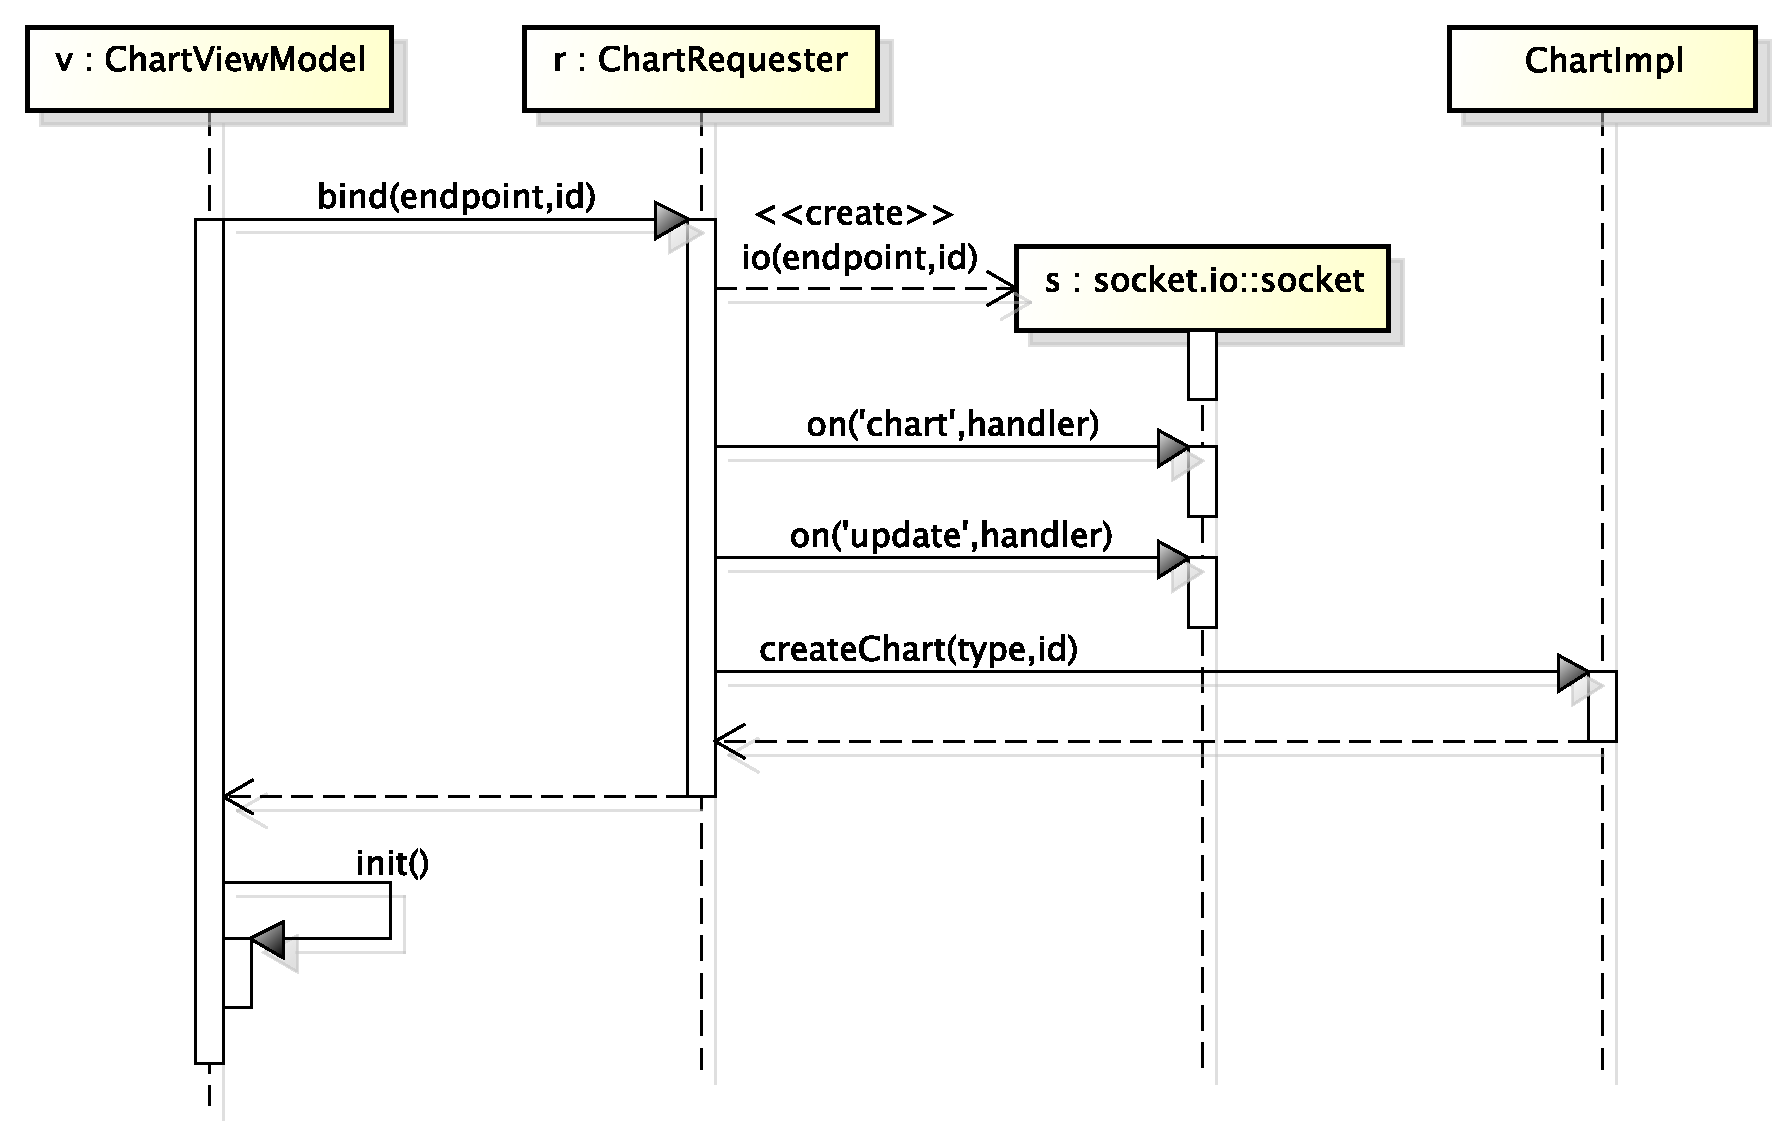
\includegraphics[scale=0.3]{DefinizioneDiProdotto/Pics/ChuckInserimentoChart}
                \caption{Diagramma di sequenza - Chuck, creazione chart}
            \end{figure}
            \begin{enumerate}
                \item ChartViewModel richiede l'ottenimento di un chart specifico presente in una istanza di \insglo{Norris} a ChartRequester;
                \item questo apre il canale socket ed imposta delle \insglo{callback} per gli eventi chart e update;
                \item ricevuto il grafico crea il modello dei dati;
                \item infine ChartViewModel esegue il metodo init che permette di inizializzare la view e visualizzare il Chart secondo i dati memorizzati.
            \end{enumerate}

        \level{3}{Aggiornamento di un chart}
            Tale diagramma descrive come viene aggiornato un chart nel momento in cui arrivano nuovi dati dall'istanza di \insglo{Norris} alla quale il grafico appartiene.
            \begin{figure}[H]
                \centering
                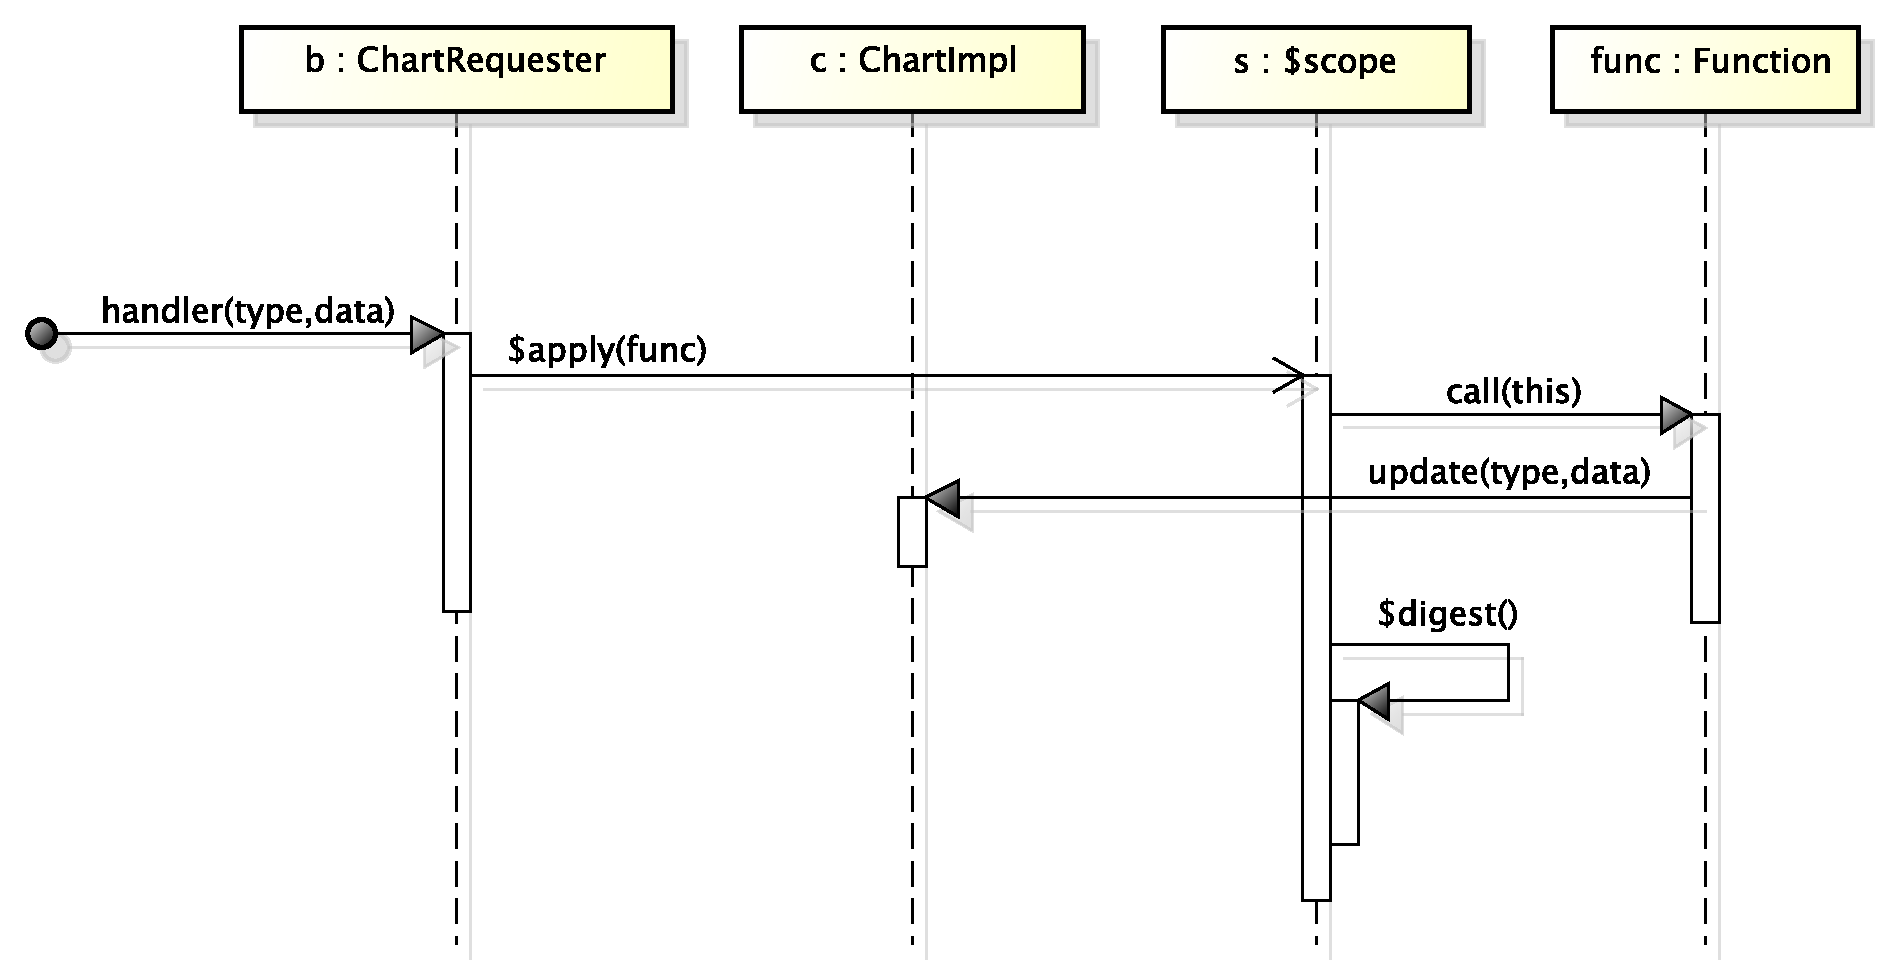
\includegraphics[scale=0.3]{DefinizioneDiProdotto/Pics/ChuckAggiornamentoChart}
                \caption{Diagramma di sequenza - Chuck, aggiornamento chart}
            \end{figure}
            \begin{enumerate}
                \item il messaggio iniziale rappresenta la notifica inviata da ChartRequester da parte di \insglo{Norris} attraverso il canale socket per avvertirlo dell'avvenuto aggiornamento;
                \item ChartRequester aggiorna il modello dei dati;
                \item avverte infine il ChartViewModel di un'avvenuta modifica nel modello richiedendo dunque la renderizzazione dei nuovi dati.
                \item
                \item
                \item
            \end{enumerate}


    \level{2}{Diagrammi di sequenza}
        In tale sezione vengono presentati i diagrammi di sequenza, che hanno lo scopo di descrivere scenari (determinate sequenze di azioni in cui tutte le scelte sono già state effettuate). Essi vengono usati per descrivere le relazioni che intercorrono, in termini di messaggi, tra attori, oggetti ed entità del sistema \insglo{Chuck}.
        \level{3}{Creazione di un chart}
             Tale diagramma riporta e descrive come viene creato un chart e collegato a quello presente all'interno di una certa istanza di \insglo{Norris}.
            \begin{figure}[H]
                \centering
                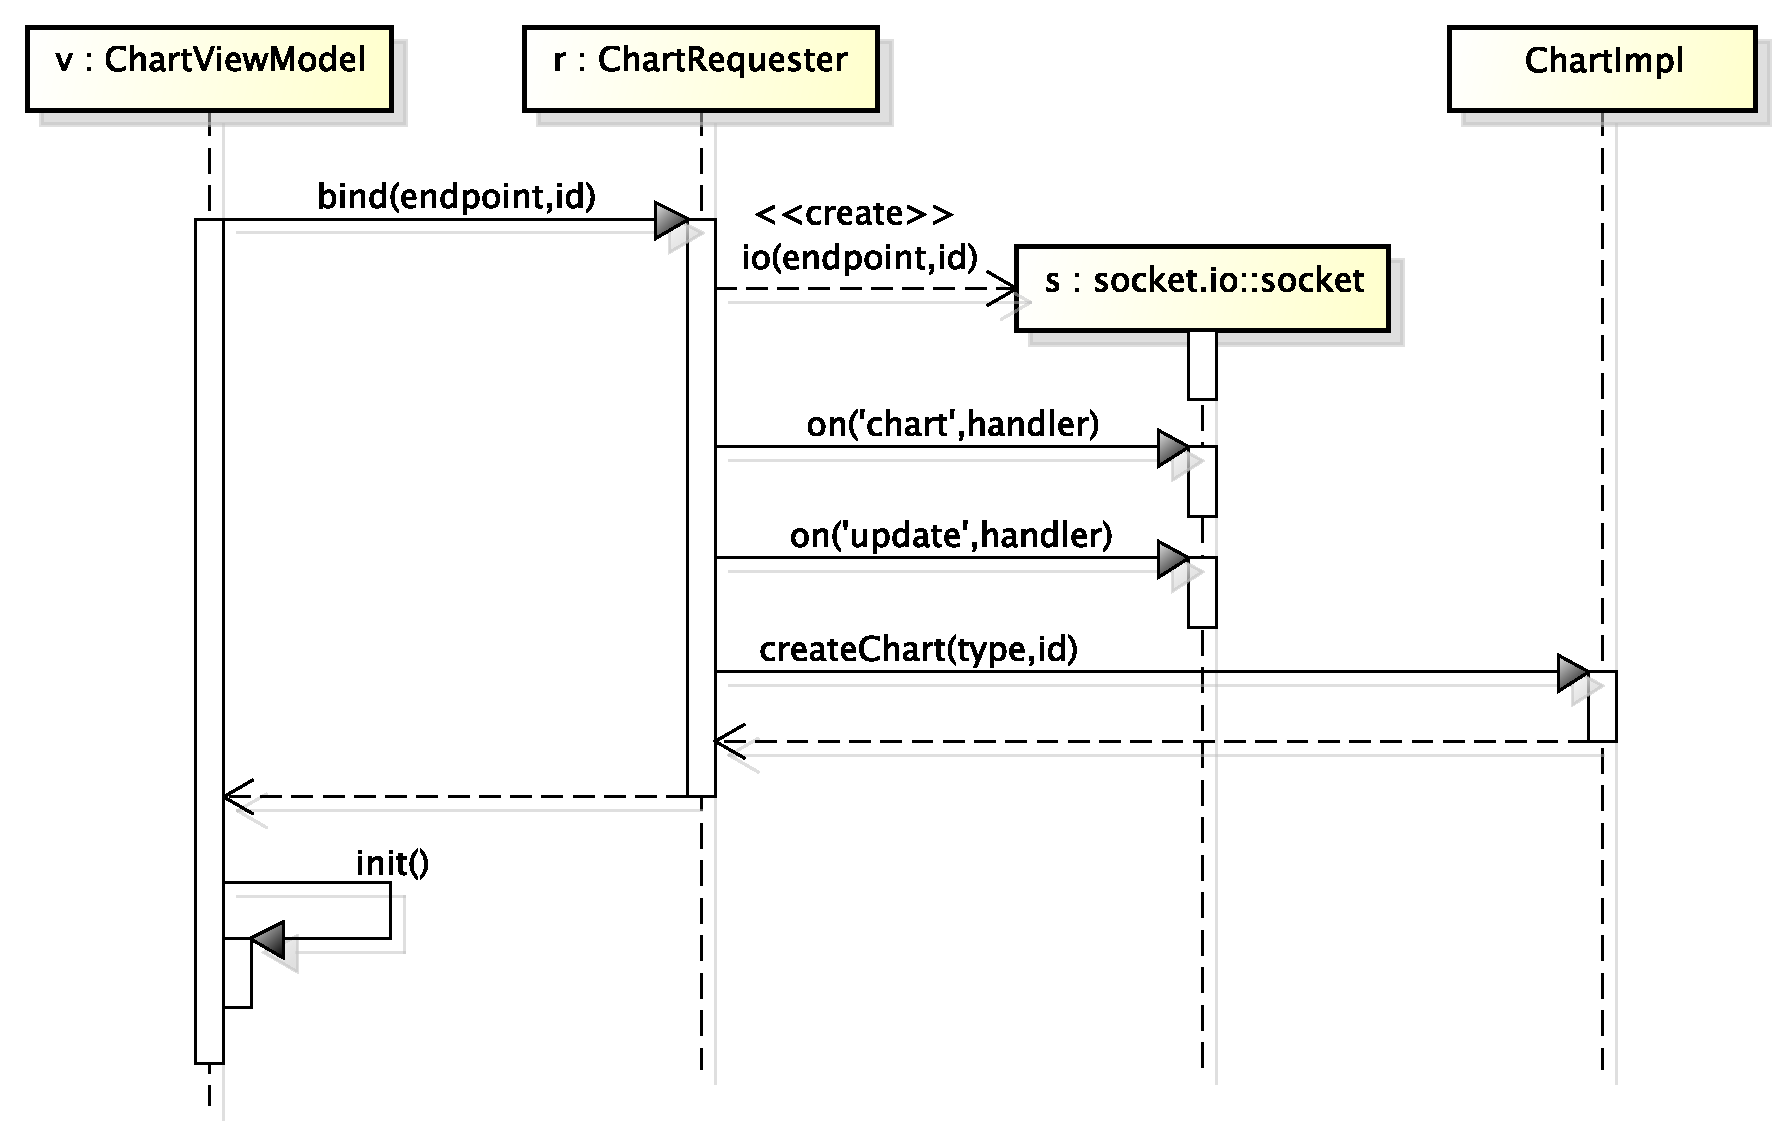
\includegraphics[scale=0.3]{DefinizioneDiProdotto/Pics/ChuckInserimentoChart}
                \caption{Diagramma di sequenza - Chuck, creazione chart}
            \end{figure}
            \begin{enumerate}
                \item ChartViewModel richiede l'ottenimento di un chart specifico presente in una istanza di \insglo{Norris} a ChartRequester;
                \item questo apre il canale socket ed imposta delle \insglo{callback} per gli eventi chart e update;
                \item ricevuto il grafico crea il modello dei dati;
                \item infine ChartViewModel esegue il metodo init che permette di inizializzare la view e visualizzare il Chart secondo i dati memorizzati.
            \end{enumerate}

        \level{3}{Aggiornamento di un chart}
            Tale diagramma descrive come viene aggiornato un chart nel momento in cui arrivano nuovi dati dall'istanza di \insglo{Norris} alla quale il grafico appartiene.
            \begin{figure}[H]
                \centering
                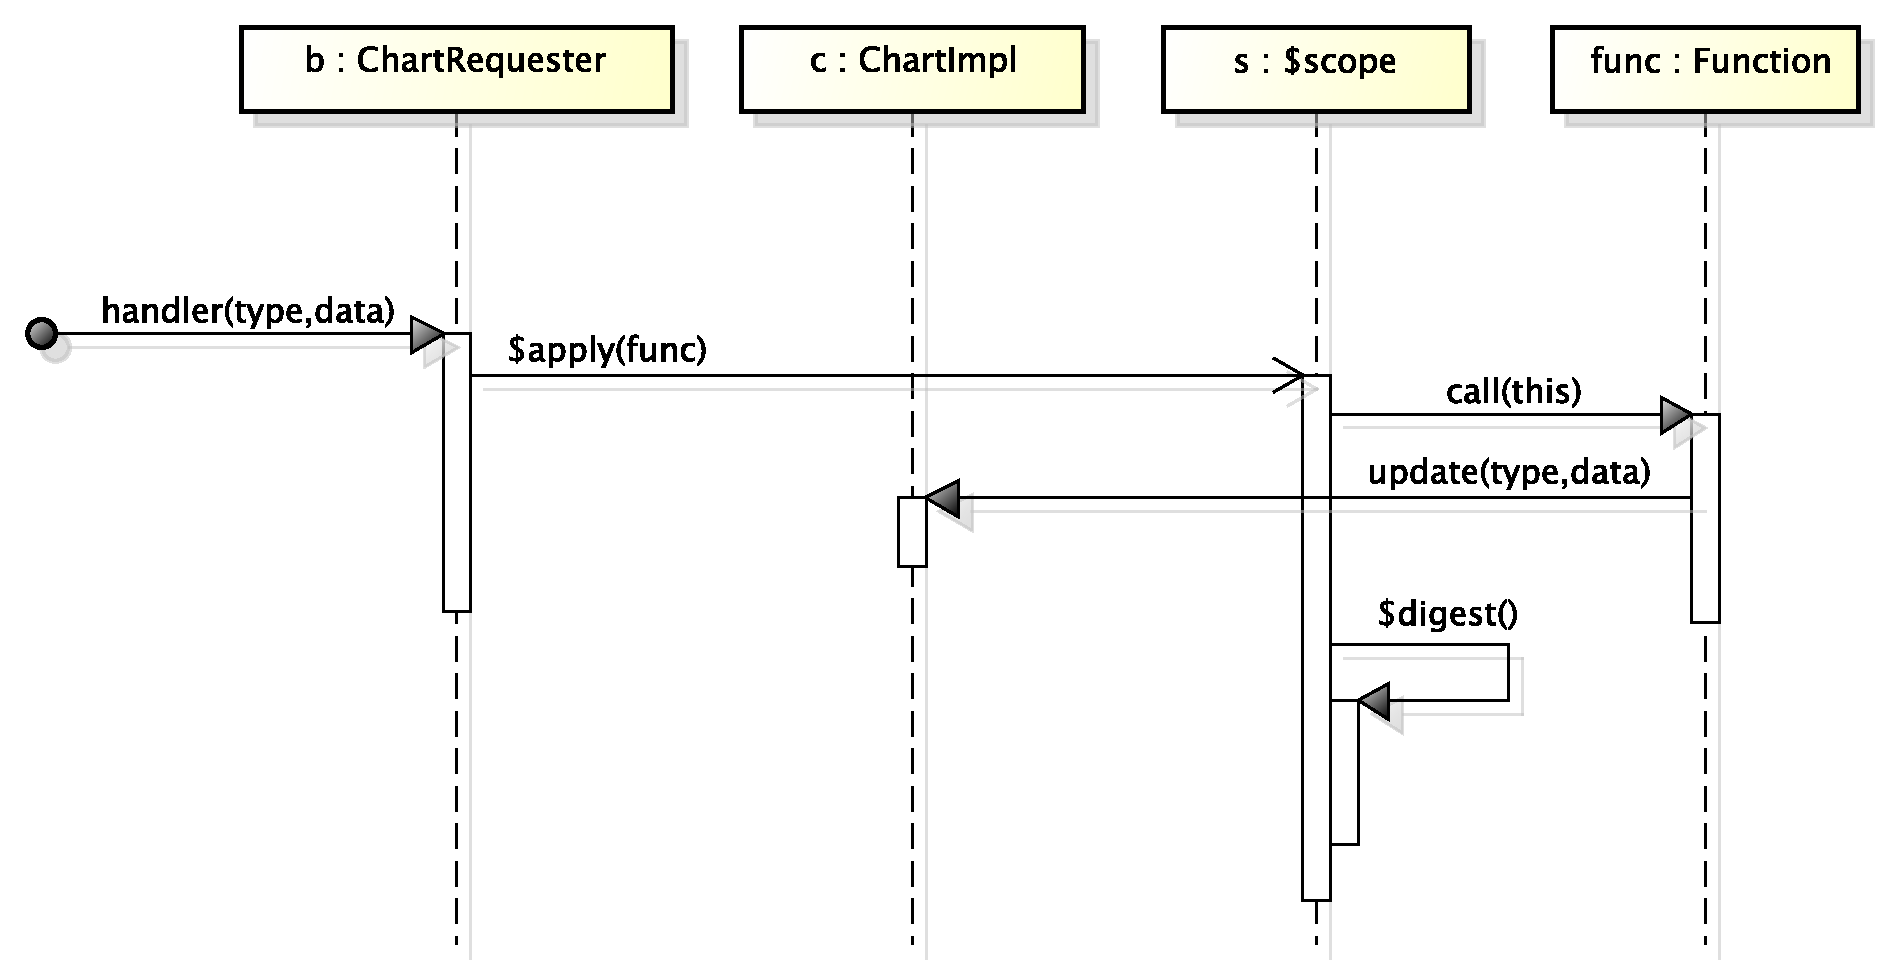
\includegraphics[scale=0.3]{DefinizioneDiProdotto/Pics/ChuckAggiornamentoChart}
                \caption{Diagramma di sequenza - Chuck, aggiornamento chart}
            \end{figure}
            \begin{enumerate}
                \item il messaggio iniziale rappresenta la notifica inviata da ChartRequester da parte di \insglo{Norris} attraverso il canale socket per avvertirlo dell'avvenuto aggiornamento;
                \item ChartRequester aggiorna il modello dei dati;
                \item avverte infine il ChartViewModel di un'avvenuta modifica nel modello richiedendo dunque la renderizzazione dei nuovi dati.
                \item
                \item
                \item
            \end{enumerate}


    \level{2}{Diagrammi di sequenza}
        In tale sezione vengono presentati i diagrammi di sequenza, che hanno lo scopo di descrivere scenari (determinate sequenze di azioni in cui tutte le scelte sono già state effettuate). Essi vengono usati per descrivere le relazioni che intercorrono, in termini di messaggi, tra attori, oggetti ed entità del sistema \insglo{Chuck}.
        \level{3}{Creazione di un chart}
             Tale diagramma riporta e descrive come viene creato un chart e collegato a quello presente all'interno di una certa istanza di \insglo{Norris}.
            \begin{figure}[H]
                \centering
                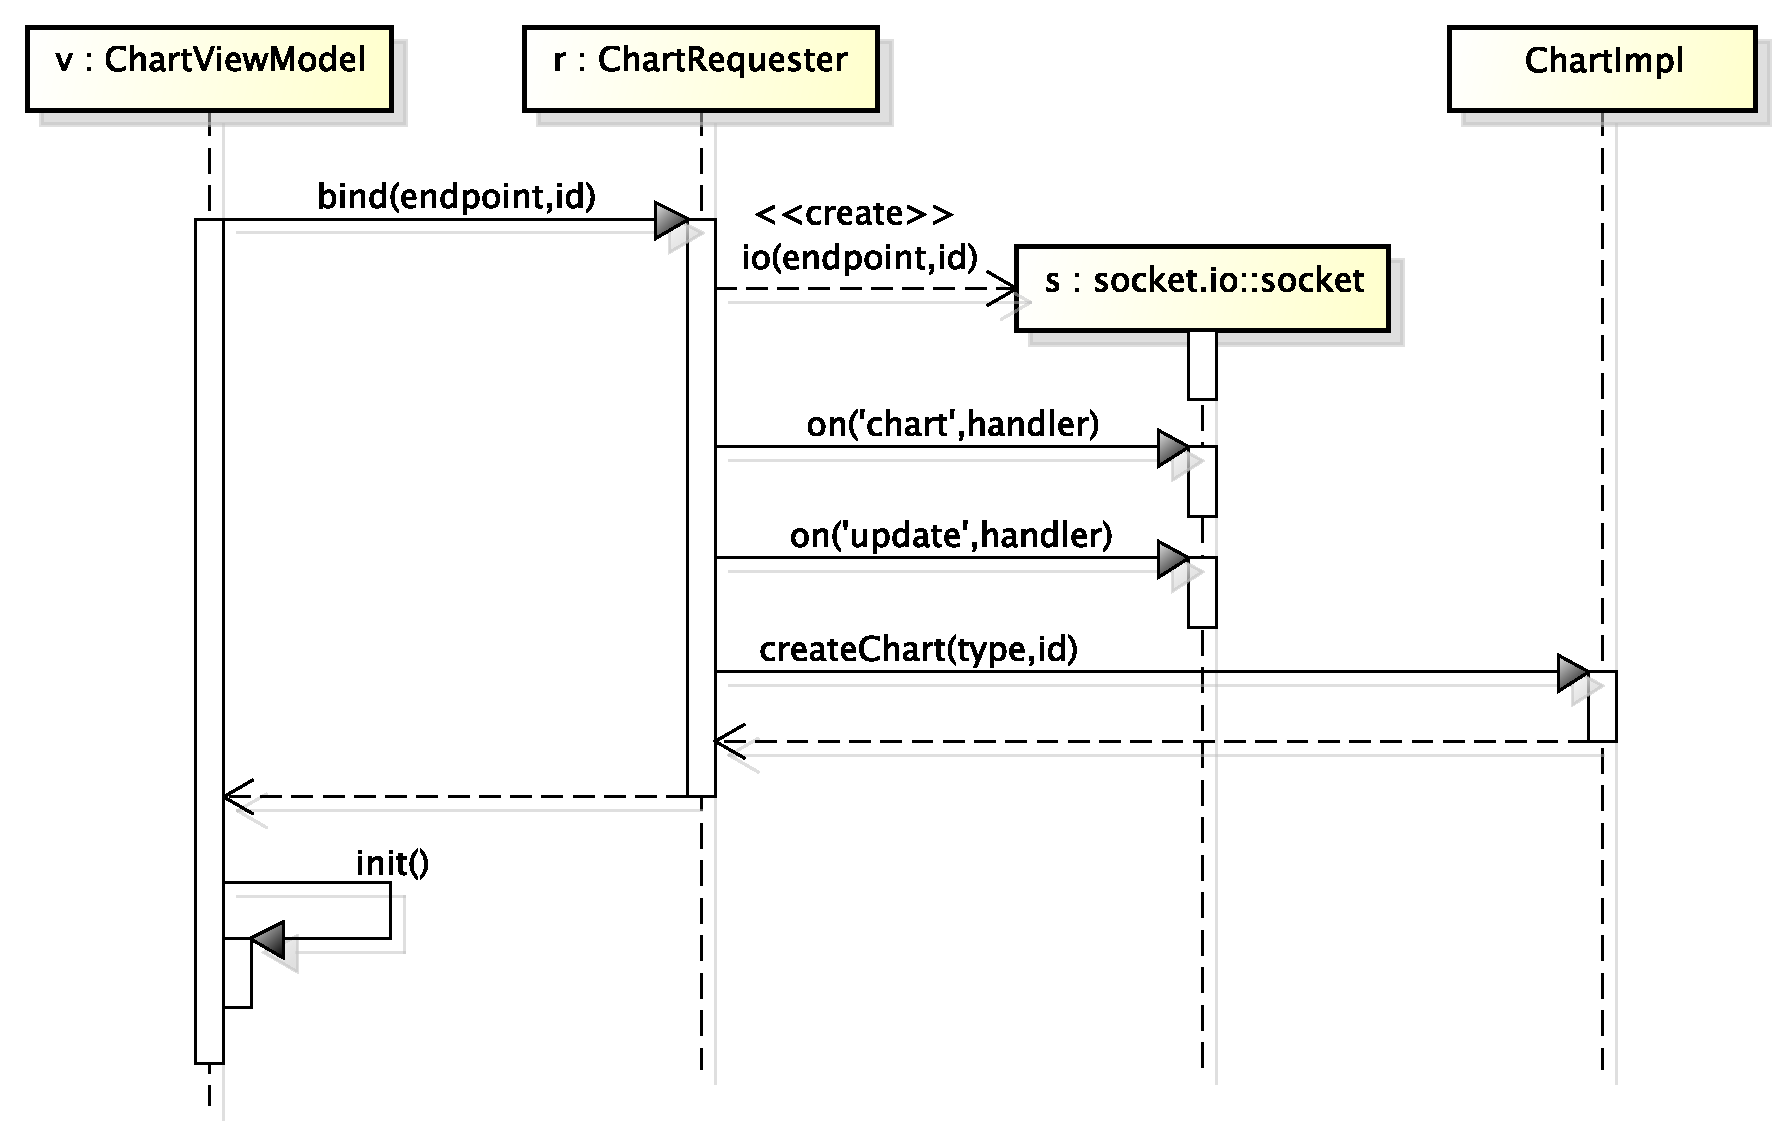
\includegraphics[scale=0.3]{DefinizioneDiProdotto/Pics/ChuckInserimentoChart}
                \caption{Diagramma di sequenza - Chuck, creazione chart}
            \end{figure}
            \begin{enumerate}
                \item ChartViewModel richiede l'ottenimento di un chart specifico presente in una istanza di Norris a ChartRequester;
                \item questo apre il canale socket ed imposta delle callback per gli eventi chart e update;
                \item ricevuto il grafico crea il modello dei dati;
                \item infine ChartViewModel esegue il metodo init che permette di inizializzare la view e visualizzare il Chart secondo i dati memorizzati.
            \end{enumerate}

        \level{3}{Aggiornamento di un chart}
            Tale diagramma descrive come viene aggiornato un chart nel momento in cui arrivano nuovi dati dall'istanza di \insglo{Norris} alla quale il grafico appartiene.
            \begin{figure}[H]
                \centering
                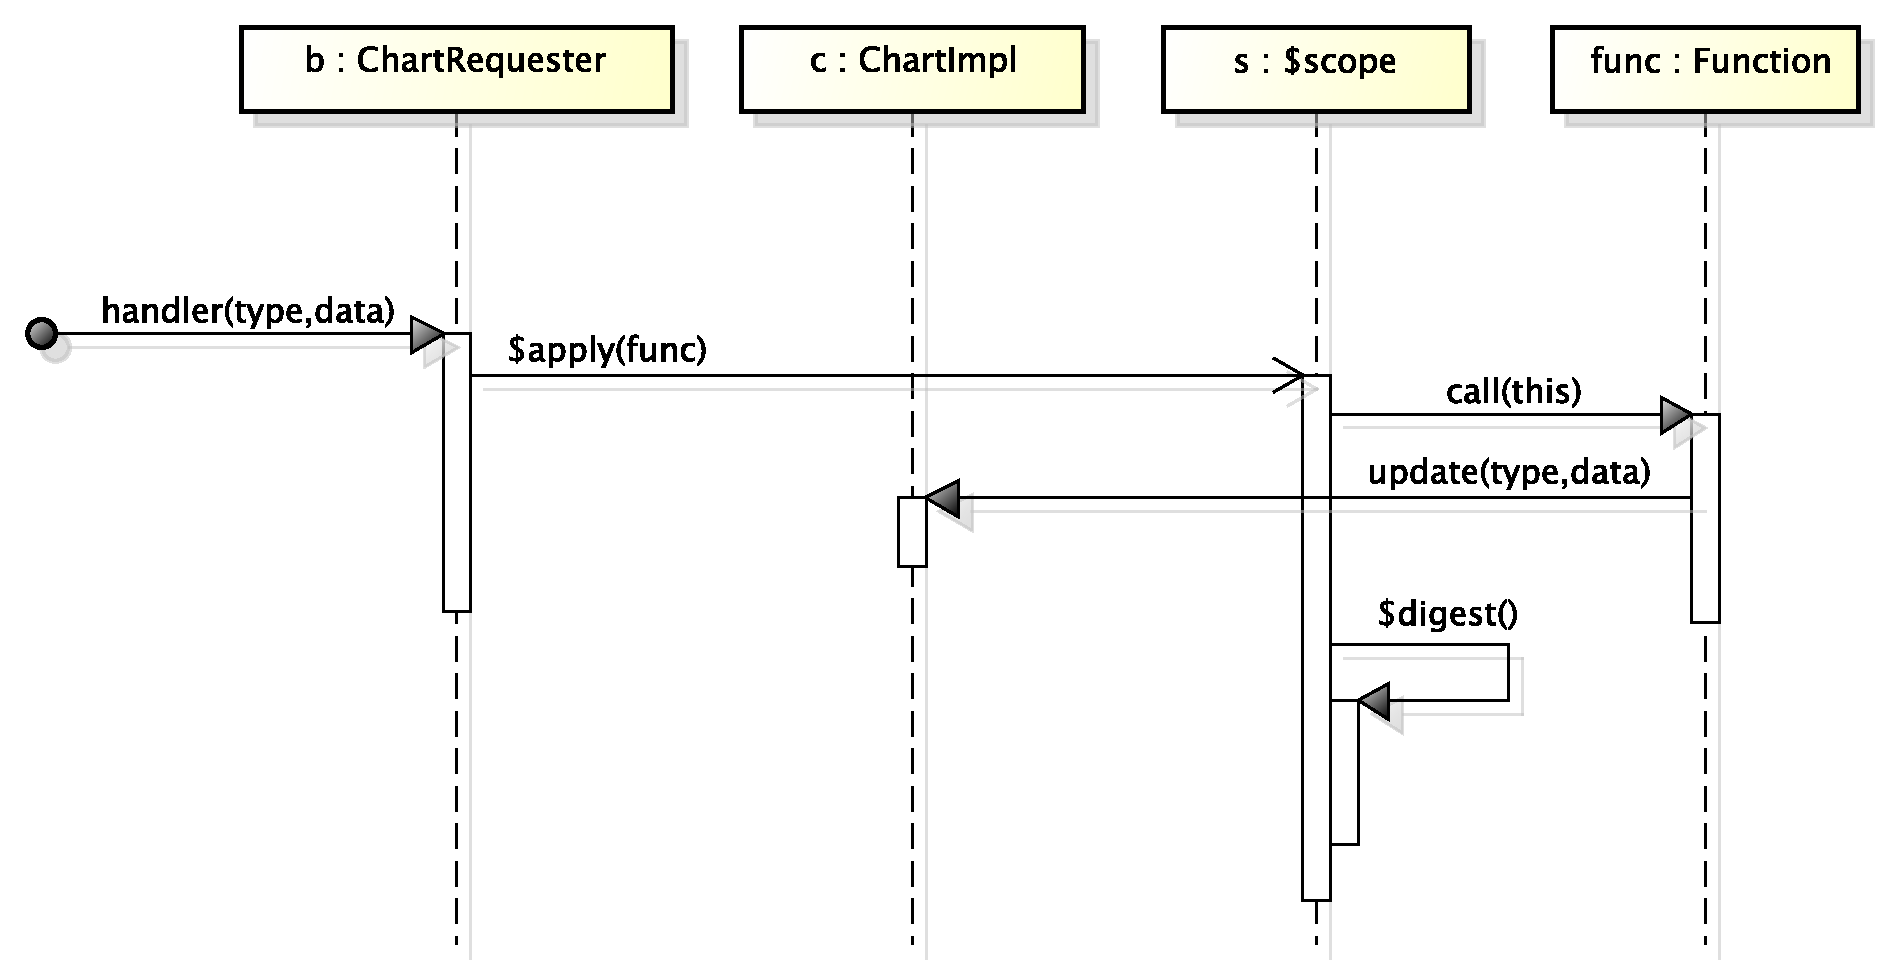
\includegraphics[scale=0.3]{DefinizioneDiProdotto/Pics/ChuckAggiornamentoChart}
                \caption{Diagramma di sequenza - Chuck, aggiornamento chart}
            \end{figure}
            \begin{enumerate}
                \item il messaggio iniziale rappresenta la notifica inviata da ChartRequester da parte di Norris attraverso il canale socket per avvertirlo dell'avvenuto aggiornamento;
                \item ChartRequester aggiorna il modello dei dati;
                \item avverte infine il ChartViewModel di un'avvenuta modifica nel modello richiedendo dunque la renderizzazione dei nuovi dati.
                \item
                \item
                \item
            \end{enumerate}
